\documentclass[preprint,12pt,authoryear]{elsarticle}

\usepackage{amsmath,amssymb,amsfonts}
\usepackage{booktabs}
\usepackage{graphicx}
\usepackage{hyperref}
\usepackage{microtype}
\usepackage{xcolor}

\setlength{\textwidth}{6.5in}
\setlength{\textheight}{9.0in}
\setlength{\oddsidemargin}{0in}
\setlength{\evensidemargin}{0in}
\setlength{\topmargin}{-0.5in}

\setcitestyle{authoryear,round,semicolon}

\hypersetup{
  colorlinks=true,
  linkcolor=blue!60!black,
  citecolor=blue!60!black,
  urlcolor=blue!60!black,
  pdftitle={Flux blindness in neural solvers for heterogeneous subsurface flow: Spectral mechanisms, pre-training screening, and flux-informed learning},
  pdfauthor={Zijie Deng, Zhenyu Liao, Jiyang Yu},
  pdfsubject={Computers & Geosciences},
  pdfcreator={LaTeX with elsarticle},
  pdfproducer={pdfTeX-1.40.25}
}

\journal{Computers \& Geosciences}

\begin{document}
\emergencystretch=2.0em

\begin{frontmatter}

\title{Flux blindness in neural solvers for heterogeneous subsurface flow: Spectral mechanisms, pre-training screening, and flux-informed learning}

\author[1]{Zijie Deng\corref{cor1}\fnref{fn1}}
\ead{3335196397vip@gmail.com}
\cortext[cor1]{Corresponding author.}
\fntext[fn1]{ORCID: 0009-0002-4824-9764.}
\author[2]{Zhenyu Liao}
\ead{2187996607@qq.com}
\author[1]{Jiyang Yu}
\ead{3488784697@qq.com}

\affiliation[1]{organization={Jiangxi Provincial Key Laboratory of Water Resources Allocation and Efficient Utilization, Jiangxi University of Water Resources and Electric Power}, addressline={No. 289 Tianxiang Avenue}, city={Nanchang}, postcode={330099}, country={China}}
\affiliation[2]{organization={School of Geography and Environment, Jiangxi Normal University}, addressline={No. 99 Ziyang Avenue}, city={Nanchang}, postcode={330022}, country={China}}

\begin{abstract}
Deep-learning surrogates for subsurface flow are conventionally trained and benchmarked on hydraulic head $h$, whereas contaminant transport and geological storage depend on the Darcy velocity $\mathbf{q} = -K\nabla h$. Here we present a reliability-aware two-stage computational workflow (\texttt{SubsurfaceReliability v1.0}) that integrates pre-training medium roughness screening, conservative face-flux operator learning, and online algebraic multigrid (AMG) residual screening and defect correction. Across $3{,}264$ held-out evaluations spanning 24 lognormal heterogeneity regimes ($\sigma^2 \in [0.5, 4.0]$, $\lambda \in [0.02, 0.20]$), 12 unseen off-grid regimes, and non-Gaussian channelized and alluvial lens media, head-trained surrogates achieve median head errors of $5.9\%$ (U-Net) and $5.5\%$ (FNO) yet exceed the zero-velocity error threshold ($E_q > 1.0$) in $91.4\%$ and $75.3\%$ of evaluations. Spectral convolution analysis and Mat\'{e}rn covariance interventions demonstrate that wavenumber-squared ($k^2$) derivative weighting amplifies high-wavenumber head residuals across rough conductivity interfaces, while controlled decoder ablations show that bilinear resize-convolution eliminates U-Net's $2.26\times$ finite-volume interface error amplification. In Stage~1, medium roughness invariants ($\sigma^2/\lambda$, $\sigma^2$, and discrete gradient energy $\mathcal{R}_{\nabla Y}$) screen regime reliability before training ($\text{ROC-AUC} = 0.915$--$0.955$; off-grid balanced accuracy $1.000$ for U-Net and $100\%$ sensitivity for FNO). Supervising FNO directly on two-point flux-approximation (TPFA) face fluxes cuts median velocity error by $52\%$--$95\%$ across Gaussian regimes and by $57\%$--$73\%$ zero-shot on channelized and alluvial lens media. In Stage~2, a single AMG V-cycle yields a reference-free residual indicator $\eta_F$ ($\text{ROC-AUC} = 0.997$), cuts median face-flux error by $93\%$ as an $O(N^2)$ defect correction, and raises Pollock advective particle breakthrough from $2.2\%$ to $94.0\%$ (median travel-time ratio $1.00$).
\end{abstract}

\begin{keyword}
Neural PDE operators \sep Heterogeneous subsurface flow \sep Fourier neural operator \sep Physics-informed neural networks \sep Finite-volume flux conservation \sep Algebraic multigrid defect correction
\end{keyword}

\end{frontmatter}

\section{Introduction}
\label{sec:intro}

Numerical simulation of fluid flow and solute transport in heterogeneous porous formations underpins groundwater management, contaminant remediation, underground hydrogen storage, and geological carbon sequestration \citep{bear1972dynamics,dagan1989flow,gelhar1993stochastic,blunt2017multiphase,lie2019mrst}. Because hydraulic conductivity $K(\mathbf{x})$ varies by orders of magnitude across spatial scales \citep{delhomme1979spatial,rubin2003applied,efendiev2013gmsfem}, ensemble data assimilation and uncertainty quantification require thousands of forward evaluations of the Darcy flow equation \citep{carrera2005inverse,laloy2012dream,chen2013ensemble,emerick2013esmda,kitanidis2014pcga}. To accelerate these multi-query workflows, deep-learning surrogates and physics-informed neural solvers have been widely adopted across computational geoscience \citep{tripathy2018deepuq,zhu2018bayesian,raissi2019pinn,mo2019deep,chang2020dl,karumuri2020simfree,tang2020dl,li2021fno,lu2021deeponet,karniadakis2021piml,lauzon2024unet}.

Three neural modeling paradigms predominate in subsurface flow computing: image-to-image convolutional encoder--decoders such as U-Net \citep{ronneberger2015unet,zhu2018bayesian,mo2019deep,chang2020dl,wang2020tgnn,lauzon2024unet}, spectral neural operators such as the Fourier neural operator (FNO) \citep{li2021fno,wen2022ufno,kovachki2023no,awr2025fvfno,awr2026benchmark}, and instance-specific physics-informed neural networks (PINNs) \citep{sirignano2018dgm,weinan2018drm,raissi2019pinn,tartakovsky2020physics,bandai2021wrr,kashefi2023pnet,cuomo2022scientific,awr2024pinn}. In standard benchmarking protocols, amortized surrogates (U-Net and FNO) are trained by minimizing the mean-squared error (MSE) on hydraulic head $h$ or pressure $p$, and model fidelity is reported via relative $L_2$ errors or $R^2$ on that state field \citep{zhu2018bayesian,mo2019deep,lu2022comprehensive}.

In subsurface hydrology and reservoir engineering, however, the primary quantity governing advective solute trajectories, capture-zone geometry, and residence times is the specific discharge (Darcy velocity) $\mathbf{q}(\mathbf{x}) = -K(\mathbf{x})\nabla h(\mathbf{x})$ \citep{raviart1977mixed,pollock1988,dagan1989flow,rubin2003applied}. Reconstructing $\mathbf{q}$ from a predicted head field $\hat{h}$ requires spatial differentiation followed by multiplication with a rough conductivity field $K(\mathbf{x}) = \exp(Y(\mathbf{x}))$. Although classical operator-norm and mixed finite-element analyses establish that $L_2$ convergence of a scalar potential does not bound its $H^1$ flux norm \citep{raviart1977mixed,ern2010posteriori}, the quantitative consequences of this decoupling in heterogeneous geological media remain poorly integrated into practical neural surrogate workflows. Recent studies have examined spectral bias in neural PDE solvers \citep{rahaman2019bias,fuks2020limits,wang2021grad,krishnapriyan2021,wang2022nntk,grossmann2024fem}, mixed pressure--velocity PINNs \citep{jagtap2020cpinn,yu2022grad,alhubail2024weight,massbal2024}, U-FNO architectures \citep{wen2022ufno}, and unsupervised finite-volume divergence losses for FNOs in mild heterogeneity ($\sigma^2 \le 0.4$) \citep{awr2025fvfno}. Nevertheless, three methodological gaps prevent reliable deployment across strong geological heterogeneity ($\sigma^2 \in [0.5, 4.0]$) and channelized or lens-dominated facies. First, practitioners lack a pre-training screening rule that predicts, directly from $K(\mathbf{x})$ before training any network, when state-only supervision fails to yield usable velocity fields. Second, the relative efficacy of unsupervised finite-volume divergence penalties versus direct supervision on harmonic face fluxes has not been isolated against matched-budget optimization controls in rough media. Third, even when derivative-aware training reduces global $L_2$ velocity error below unity, residual cell-level divergence errors can still sever advective streamlines, necessitating a reference-free online diagnostic and fast conservative correction.

Here we develop a unified, reliability-aware two-stage computational workflow (\texttt{SubsurfaceReliability v1.0}) that resolves these gaps by linking spectral operator-norm diagnosis, pre-training medium roughness screening (Stage~1), conservative two-point flux-approximation (TPFA) face-flux operator training, and online single-cycle algebraic multigrid (AMG) residual screening and defect correction (Stage~2). We formalize the regime of \textit{flux blindness}, in which a solver achieves low relative $L_2$ head error ($E_h \approx 5\%$--$6\%$) while its derived Darcy velocity field exceeds unit relative error ($E_q > 1.0$, worse than predicting zero flow $\hat{\mathbf{q}} = \mathbf{0}$). Using a verified benchmark suite spanning 24 lognormal regimes ($3{,}264$ evaluations), 12 prospective off-grid blind regimes, and non-Gaussian channelized and Macrodispersion Experiment (MADE)-type alluvial lens media, we establish the spectral mechanism of state--velocity decoupling, validate transferable pre-training screening rules, demonstrate why direct TPFA face-flux supervision outperforms unsupervised divergence penalties, and quantify the accuracy--cost trade-offs of hybrid neural--AMG defect correction for advective transport.

\section{Computational Workflow and Experimental Design}
\label{sec:methods}

Our computational framework (\texttt{SubsurfaceReliability v1.0}) is structured around the four-stage verification and evaluation pipeline summarized in Table~\ref{tab:workflow_specs}. Full hyperparameter sensitivity checks, vector-norm comparisons, and multi-seed tables are provided in the Supplementary Material.

\begin{table}[t!]
\centering
\caption{Summary of solver architectures, spatial representations, training protocols, and evaluation metrics in the \texttt{SubsurfaceReliability v1.0} workflow.}
\label{tab:workflow_specs}
\resizebox{\textwidth}{!}{%
\begin{tabular}{p{2.5cm}p{3.0cm}p{3.2cm}p{3.2cm}p{3.2cm}}
\toprule
\textbf{Component} & \textbf{TPFA Reference} & \textbf{Convolutional U-Net} & \textbf{Fourier Operator (FNO)} & \textbf{Coordinate PINN} \\
\midrule
Paradigm & Direct FV solver & Amortized 2D CNN & Amortized spectral net & Per-instance MLP \\
Input tensor & Cell $K_{i,j}$ ($128^2, 256^2$) & $[Y_{\text{std}}, x, y] \in \mathbb{R}^{3\times N\times N}$ & $[Y_{\text{std}}, x, y] \in \mathbb{R}^{3\times N\times N}$ & $(x,y) \in [0,1]^2$; $4N$ $(Y,\nabla Y)$ \\
Architecture & Harmonic face $T_{i+1/2,j}$ & $w=24$, $d=3$, GroupNorm & $w=24$, $L=4$, $m=12$ modes & $4\times 64$ $\tanh$; hard BC \\
Parameters & None ($A_K \mathbf{h} = \mathbf{b}$) & $263{,}689$ (Resize: $292{,}489$) & $669{,}377$ tensor elements & $12{,}737$ per realization \\
Objective & Exact $\nabla_h\cdot\mathbf{F}=0$ & $\mathcal{L}_h$ or $\mathcal{L}_h + (\alpha/f_0)\mathcal{L}_q$ & $\mathcal{L}_h$ or $\mathcal{L}_h + (\alpha/f_0)\mathcal{L}_q$ & PDE residual ($r_{\text{norm}}$ or $K r$) \\
Optimization & Direct LU ($41\text{ ms}$) & Adam ($80$ ep, lr $10^{-3}$) & Adam ($80$ ep, lr $10^{-3}$) & $10{,}000$ Adam + $500$ L-BFGS \\
Data split/cell & $352$ realizations & $128$ train / $32$ val / $64$ test & $128$ train / $32$ val / $64$ test & $8$ stratified test instances \\
Evaluations & MMS + $256^2$ check & $1{,}536$ atlas + $832$ o.o.d. & $1{,}536$ atlas + $832$ o.o.d. & $192$ atlas + $8$ blind \\
Diagnostics & Reference ($E_q=0$) & $E_h, E_q, E_{q,\text{face}}, \mathcal{I}_{\text{div}}, \eta_F$ & $E_h, E_q, E_{q,\text{face}}, \mathcal{I}_{\text{div}}, \eta_F$ & $E_h, E_q, E_{q,\text{face}}, \mathcal{I}_{\text{div}}, \eta_F$ \\
\bottomrule
\end{tabular}%
}
\end{table}

\subsection{Governing Equations and Spectral Medium Synthesis}
\label{sec:governing}

We consider steady-state, single-phase Darcy flow on the dimensionless unit square $\Omega = [0, L]^2$ ($L = 1$):
\begin{equation}
  -\nabla \cdot \big(K(\mathbf{x})\nabla h(\mathbf{x})\big) = 0, \quad \mathbf{x} = (x, y) \in \Omega,
  \label{eq:darcy_pde}
\end{equation}
where $h(\mathbf{x})$ is dimensionless hydraulic head and $\mathbf{q}(\mathbf{x}) = -K(\mathbf{x})\nabla h(\mathbf{x})$ is the Darcy velocity, subject to Dirichlet inflow/outflow and lateral no-flow boundary conditions:
\begin{equation}
  h(0, y) = 1, \quad h(1, y) = 0, \quad \frac{\partial h}{\partial y}(x, 0) = \frac{\partial h}{\partial y}(x, 1) = 0.
  \label{eq:bcs}
\end{equation}
In the primary 24-regime benchmark atlas, hydraulic conductivity is modeled as a lognormal field $K(\mathbf{x}) = \exp(Y(\mathbf{x}))$ \citep{dagan1989flow,gelhar1993stochastic,dietrich1993fast}, where $Y(\mathbf{x}) = \ln K(\mathbf{x})$ is a zero-mean Gaussian field with variance $\sigma^2$, dimensionless correlation length $\lambda$, and isotropic Gaussian autocovariance:
\begin{equation}
  C_Y(r) = \sigma^2 \exp\!\left(-\frac{r^2}{2\lambda^2}\right), \quad r = \|\mathbf{x} - \mathbf{x}'\|_2,
  \label{eq:gauss_cov}
\end{equation}
having analytical radial integral scale $I_Y = \lambda\sqrt{\pi/2}$. To ensure exact physical equivalence between grid-based operators and continuous coordinate networks, each realization $Y(\mathbf{x})$ is synthesized via its exact band-limited trigonometric Fourier expansion with zero mean and exact sample variance $\sigma^2$. Grid solvers evaluate $Y(\mathbf{x})$ at the $N \times N$ cell centers ($N = 128$, and $N = 256$ in the resolution-scaling benchmark), whereas the PINN queries bilinear interpolants of exact spectral $(Y, \partial_x Y, \partial_y Y)$ fields precomputed on a $4N \times 4N$ grid (interpolation error $4 \times 10^{-7}$).

To isolate small-scale roughness at fixed variance $\sigma^2$ and fixed integral scale $I_Y = \lambda\sqrt{\pi/2}$, we also construct controlled Mat\'{e}rn covariance interventions with smoothness $\nu = 3/2$ and $\nu = 1/2$ \citep{rubin2003applied}:
\begin{equation}
  C_{\nu=3/2}(r) = \sigma^2 \left(1 + \frac{r}{\ell_{3/2}}\right)\exp\!\left(-\frac{r}{\ell_{3/2}}\right), \quad
  C_{\nu=1/2}(r) = \sigma^2 \exp\!\left(-\frac{r}{\ell_{1/2}}\right),
  \label{eq:matern_cov}
\end{equation}
with $\ell_{3/2} = I_Y / 2$ and $\ell_{1/2} = I_Y$, quantifying high-wavenumber energy via the spectral fraction $\Phi(k_c = 8) = E_Y(k \ge 8) / E_{Y,\text{tot}}$. Beyond multi-Gaussian fields, we evaluate two non-Gaussian hydrofacies ensembles on $128 \times 128$ grids ($16$ realizations per regime): (i) sinuous binary-facies channelized aquifers ($35\%$ connected high-$K$ channels across $\sigma^2 \in \{0.5, 1.0, 2.0\}$) and (ii) strongly heterogeneous three-facies alluvial cross-sections ($\sigma^2 = 4.5$, gravel conduits, sand matrix, and silt-clay lenses with anisotropy $\lambda_x = 0.22, \lambda_z = 0.03$) modeled after the Macrodispersion Experiment (MADE) aquifer \citep{zheng2011made}.

\subsection{Verified Finite-Volume Reference Solver and Atlas Design}
\label{sec:fv_solver}

Reference solutions are computed using a locally conservative cell-centered TPFA finite-volume scheme \citep{eymard2000}. Across adjacent cells, the normal face flux is governed by harmonic transmissibility weighting:
\begin{equation}
  F_{i+1/2, j} = -T_{i+1/2, j}\,\frac{h_{i+1, j} - h_{i, j}}{\Delta x}, \quad
  T_{i+1/2, j} = \frac{2 K_{i, j} K_{i+1, j}}{K_{i, j} + K_{i+1, j}},
  \label{eq:tpfa}
\end{equation}
yielding a symmetric positive-definite system $A_K \mathbf{h} = \mathbf{b}$ solved via sparse direct factorization. Automated verification gates (\texttt{src/subrel/verify.py}) confirm second-order convergence ($2.00$ in head, $1.98$ in flux) under the method of manufactured solutions \citep{roache1998}, exact linear head recovery ($1.0 \times 10^{-14}$), and machine-precision cell divergence closure ($\le 8.6 \times 10^{-12}$). Grid-refinement checks between $128^2$ and $256^2$ grids confirm that discretization differences ($0.03\%$--$6.1\%$ across the Gaussian atlas) are an order of magnitude smaller than neural flux errors (Supplementary Section~S1).

The full-factorial atlas spans $\sigma^2 \in \{0.5, 1.0, 2.0, 4.0\} \times \lambda \in \{0.02, 0.03, 0.05, 0.08, 0.12, 0.20\}$ ($24$ regimes, each with $128$ baseline training, $128$ reserve training, $32$ validation, and $64$ held-out test realizations). Evaluating U-Net and FNO across all $64$ test realizations per cell ($1{,}536$ evaluations each) and per-instance PINNs across the first $8$ test realizations per cell ($192$ evaluations) yields $3{,}264$ primary atlas evaluations, complemented by 12 off-grid blind regimes ($768$ test realizations).

\subsection{Neural Solver Architectures and Training Protocols}
\label{sec:solvers}

All baseline solvers use uniform hyperparameters across regimes (Table~\ref{tab:workflow_specs}). The baseline 2D U-Net \citep{ronneberger2015unet} maps $[Y_{\text{std}}(\mathbf{x}), x, y] \in \mathbb{R}^{3 \times N \times N}$ to normalized head $\tilde{h} = 2\hat{h} - 1$ using base width $w = 24$, three resolution levels ($24 \to 48 \to 96$), $2 \times 2$ average pooling, and stride-2 transposed-convolution upsampling ($263{,}689$ parameters). To isolate decoder-induced interface oscillations, we also evaluate a controlled variant (\texttt{ResizeUNet}, $292{,}489$ parameters) that replaces stride-2 transposed convolutions with bilinear upsampling followed by a $3 \times 3$ convolution. The 2D FNO \citep{li2021fno} lifts $[Y_{\text{std}}(\mathbf{x}), x, y]$ to width $w = 24$ followed by $L = 4$ spectral convolution layers retaining $m_1 = m_2 = 12$ Fourier modes ($669{,}377$ parameter elements). Both amortized families are trained on $128$ realizations for $80$ epochs (batch size $32$, Adam learning rate $10^{-3}$ with cosine annealing) using validation early stopping.

The per-instance coordinate PINN \citep{raissi2019pinn} ($4 \times 64$ $\tanh$ layers, $12{,}737$ parameters) enforces the Dirichlet conditions exactly via the hard trial ansatz \citep{lu2021pinn}:
\begin{equation}
  \hat{h}(x, y; \theta) = (1 - x) + x(1 - x)\,\mathcal{N}_\theta(x, y),
  \label{eq:hard_bc}
\end{equation}
and minimizes the conductivity-normalized residual:
\begin{equation}
  r(x, y; \theta) = \Delta\hat{h}(x, y; \theta) + \nabla Y(x, y) \cdot \nabla\hat{h}(x, y; \theta),
  \label{eq:pinn_res}
\end{equation}
plus a lateral Neumann penalty over $M = 16{,}384$ Latin-hypercube interior collocation points and $M_{\text{bc}} = 1{,}024$ boundary points for $10{,}000$ Adam iterations followed by $500$ L-BFGS steps. We also evaluate residual-adaptive resampling (RAR) \citep{lu2021deepxde} and conductivity-weighted residuals $K(\Delta\hat{h} + \nabla Y \cdot \nabla\hat{h})$ in Section~\ref{sec:repairs_results}.

\subsection{Evaluation Metrics and Streamline Transport Protocol}
\label{sec:metrics}

All error metrics are evaluated on the interior domain $\Omega_{\text{int}}$ excluding a 2-cell boundary margin. The relative $L_2$ hydraulic-head error and Darcy velocity error are defined as
\begin{equation}
  E_h = \frac{\|\hat{h} - h\|_{2, \Omega_{\text{int}}}}{\|h\|_{2, \Omega_{\text{int}}}},
  \label{eq:eh}
\end{equation}
\begin{equation}
  E_q = \frac{\|\hat{q}_x - q_x\|_{2, \Omega_{\text{int}}} + \|\hat{q}_y - q_y\|_{2, \Omega_{\text{int}}}}{\|q_x\|_{2, \Omega_{\text{int}}} + \|q_y\|_{2, \Omega_{\text{int}}}},
  \label{eq:eq}
\end{equation}
and the conservative TPFA face-flux error $E_{q,\text{face}}$ is defined analogously on the interior cell faces using Eq.~\eqref{eq:tpfa}. A velocity prediction is classified as a \textit{flux failure} when $E_q > 1.0$ (worse than predicting $\hat{\mathbf{q}} = \mathbf{0}$); replacing Eq.~\eqref{eq:eq} with the joint Euclidean vector norm alters only $5.2\%$ of binary classifications across all $3{,}072$ amortized evaluations and leaves all screening rules unchanged (Supplementary Section~S2). Local mass-balance violation is quantified by the dimensionless divergence imbalance:
\begin{equation}
  \mathcal{I}_{\text{div}} = \frac{\|\nabla_h \cdot \hat{\mathbf{q}}_f\|_{2, \Omega_{\text{int}}}}{(\|q_{f,x}\|_{2, \Omega_{\text{int}}} + \|q_{f,y}\|_{2, \Omega_{\text{int}}}) / \Delta x}.
  \label{eq:idiv}
\end{equation}
Downstream advective solute transport is evaluated via semi-analytical Pollock streamline tracking \citep{pollock1988} on the reconstructed TPFA face fluxes across $24$ test realizations ($41$ particles released at $x = 2\Delta x$ per realization, $984$ trajectories per solver) spanning $(\sigma^2, \lambda) \in \{(0.5, 0.08), (1.0, 0.05), (2.0, 0.03)\}$, recording whether each trajectory arrives at the outlet ($x = 1 - 2\Delta x$), stalls in an artificial interior sink cell, or exits backward through the inflow boundary.

\section{Results}
\label{sec:results}

\subsection{The Empirical Reliability Atlas and State--Velocity Decoupling}
\label{sec:atlas_results}

Across all 24 heterogeneity regimes ($3{,}264$ held-out evaluations), head-trained amortized surrogates achieve high accuracy on the state variable $h$, with pooled median head errors of $5.9\%$ for U-Net and $5.5\%$ for FNO, whereas the per-instance PINN exhibits a larger median head error of $27.1\%$ due to optimization stiffness in rough media (Table~\ref{tab:atlas_summary}; Figure~\ref{fig:phase}). When evaluated on the derived Darcy velocity $\mathbf{q} = -K\nabla h$, however, the performance ranking reverses. Despite head errors below $6\%$, the baseline U-Net yields a pooled median flux error of $E_q = 2.75$, exceeding the zero-velocity threshold $E_q = 1.0$ in $91.4\%$ of realizations and achieving regime-median skill ($E_q \le 1.0$) in only $1/24$ regimes ($\sigma^2 = 0.5, \lambda = 0.20$). The baseline FNO yields a pooled median flux error of $E_q = 1.71$ ($75.3\%$ failure rate), maintaining regime-median skill in $7/24$ regimes (all six $\sigma^2 = 0.5$ cells plus $(1.0, 0.20)$). By contrast, the per-instance PINN achieves a pooled median flux error of $0.90$ and satisfies $E_q \le 1.0$ in $14/24$ regimes.

\begin{table}[t!]
\centering
\caption{Atlas-wide performance summary across 24 lognormal heterogeneity regimes ($3{,}264$ held-out evaluations). Note on computational budget: U-Net and FNO are amortized surrogates trained once per regime ($95$--$110\text{ s}$) and evaluated in a single forward pass ($2.8\text{ ms/realization}$) across $64$ test instances/cell, whereas PINN is an instance-specific PDE optimizer ($10{,}500$ steps, $\sim 95\text{ s/realization}$) evaluated on $8$ stratified test instances/cell. Cell-cluster bootstrap 95\% confidence intervals ($1{,}000$ resamples) are reported for each family's governing pre-training ROC-AUC predictor.}
\label{tab:atlas_summary}
\resizebox{\textwidth}{!}{%
\begin{tabular}{lccccccc}
\toprule
\textbf{Solver Family (Paradigm, Test $N$)} & \textbf{Med.\ $E_h$} & \textbf{95th $E_h$} & \textbf{Med.\ $E_q$} & \textbf{Fail Rate} & \textbf{Med.\ $E_{q,\text{face}}$} & \textbf{Med.\ $\mathcal{I}_{\text{div}}$} & \textbf{Pre-Train AUC [95\% CI]} \\
\midrule
U-Net (amortized, $1{,}536$, $1/24$ pass) & 5.9\% & 15.7\% & 2.75 & 91.4\% & 5.48 & 8.27 & $\sigma^2/\lambda$: $0.955$ [$0.887, 0.980$] \\
FNO (amortized, $1{,}536$, $7/24$ pass)   & 5.5\% & 15.2\% & 1.71 & 75.3\% & 1.67 & 1.01 & $\sigma^2$: $0.915$ [$0.844, 0.953$] \\
PINN (per-instance, $192$, $14/24$ pass)  & 27.1\% & 65.5\% & 0.90 & 44.3\% & 0.98 & 0.03 & $\sigma^2/\lambda^2$: $0.938$ [$0.865, 0.979$] \\
\bottomrule
\end{tabular}%
}
\end{table}

\begin{figure}[t!]
\centering
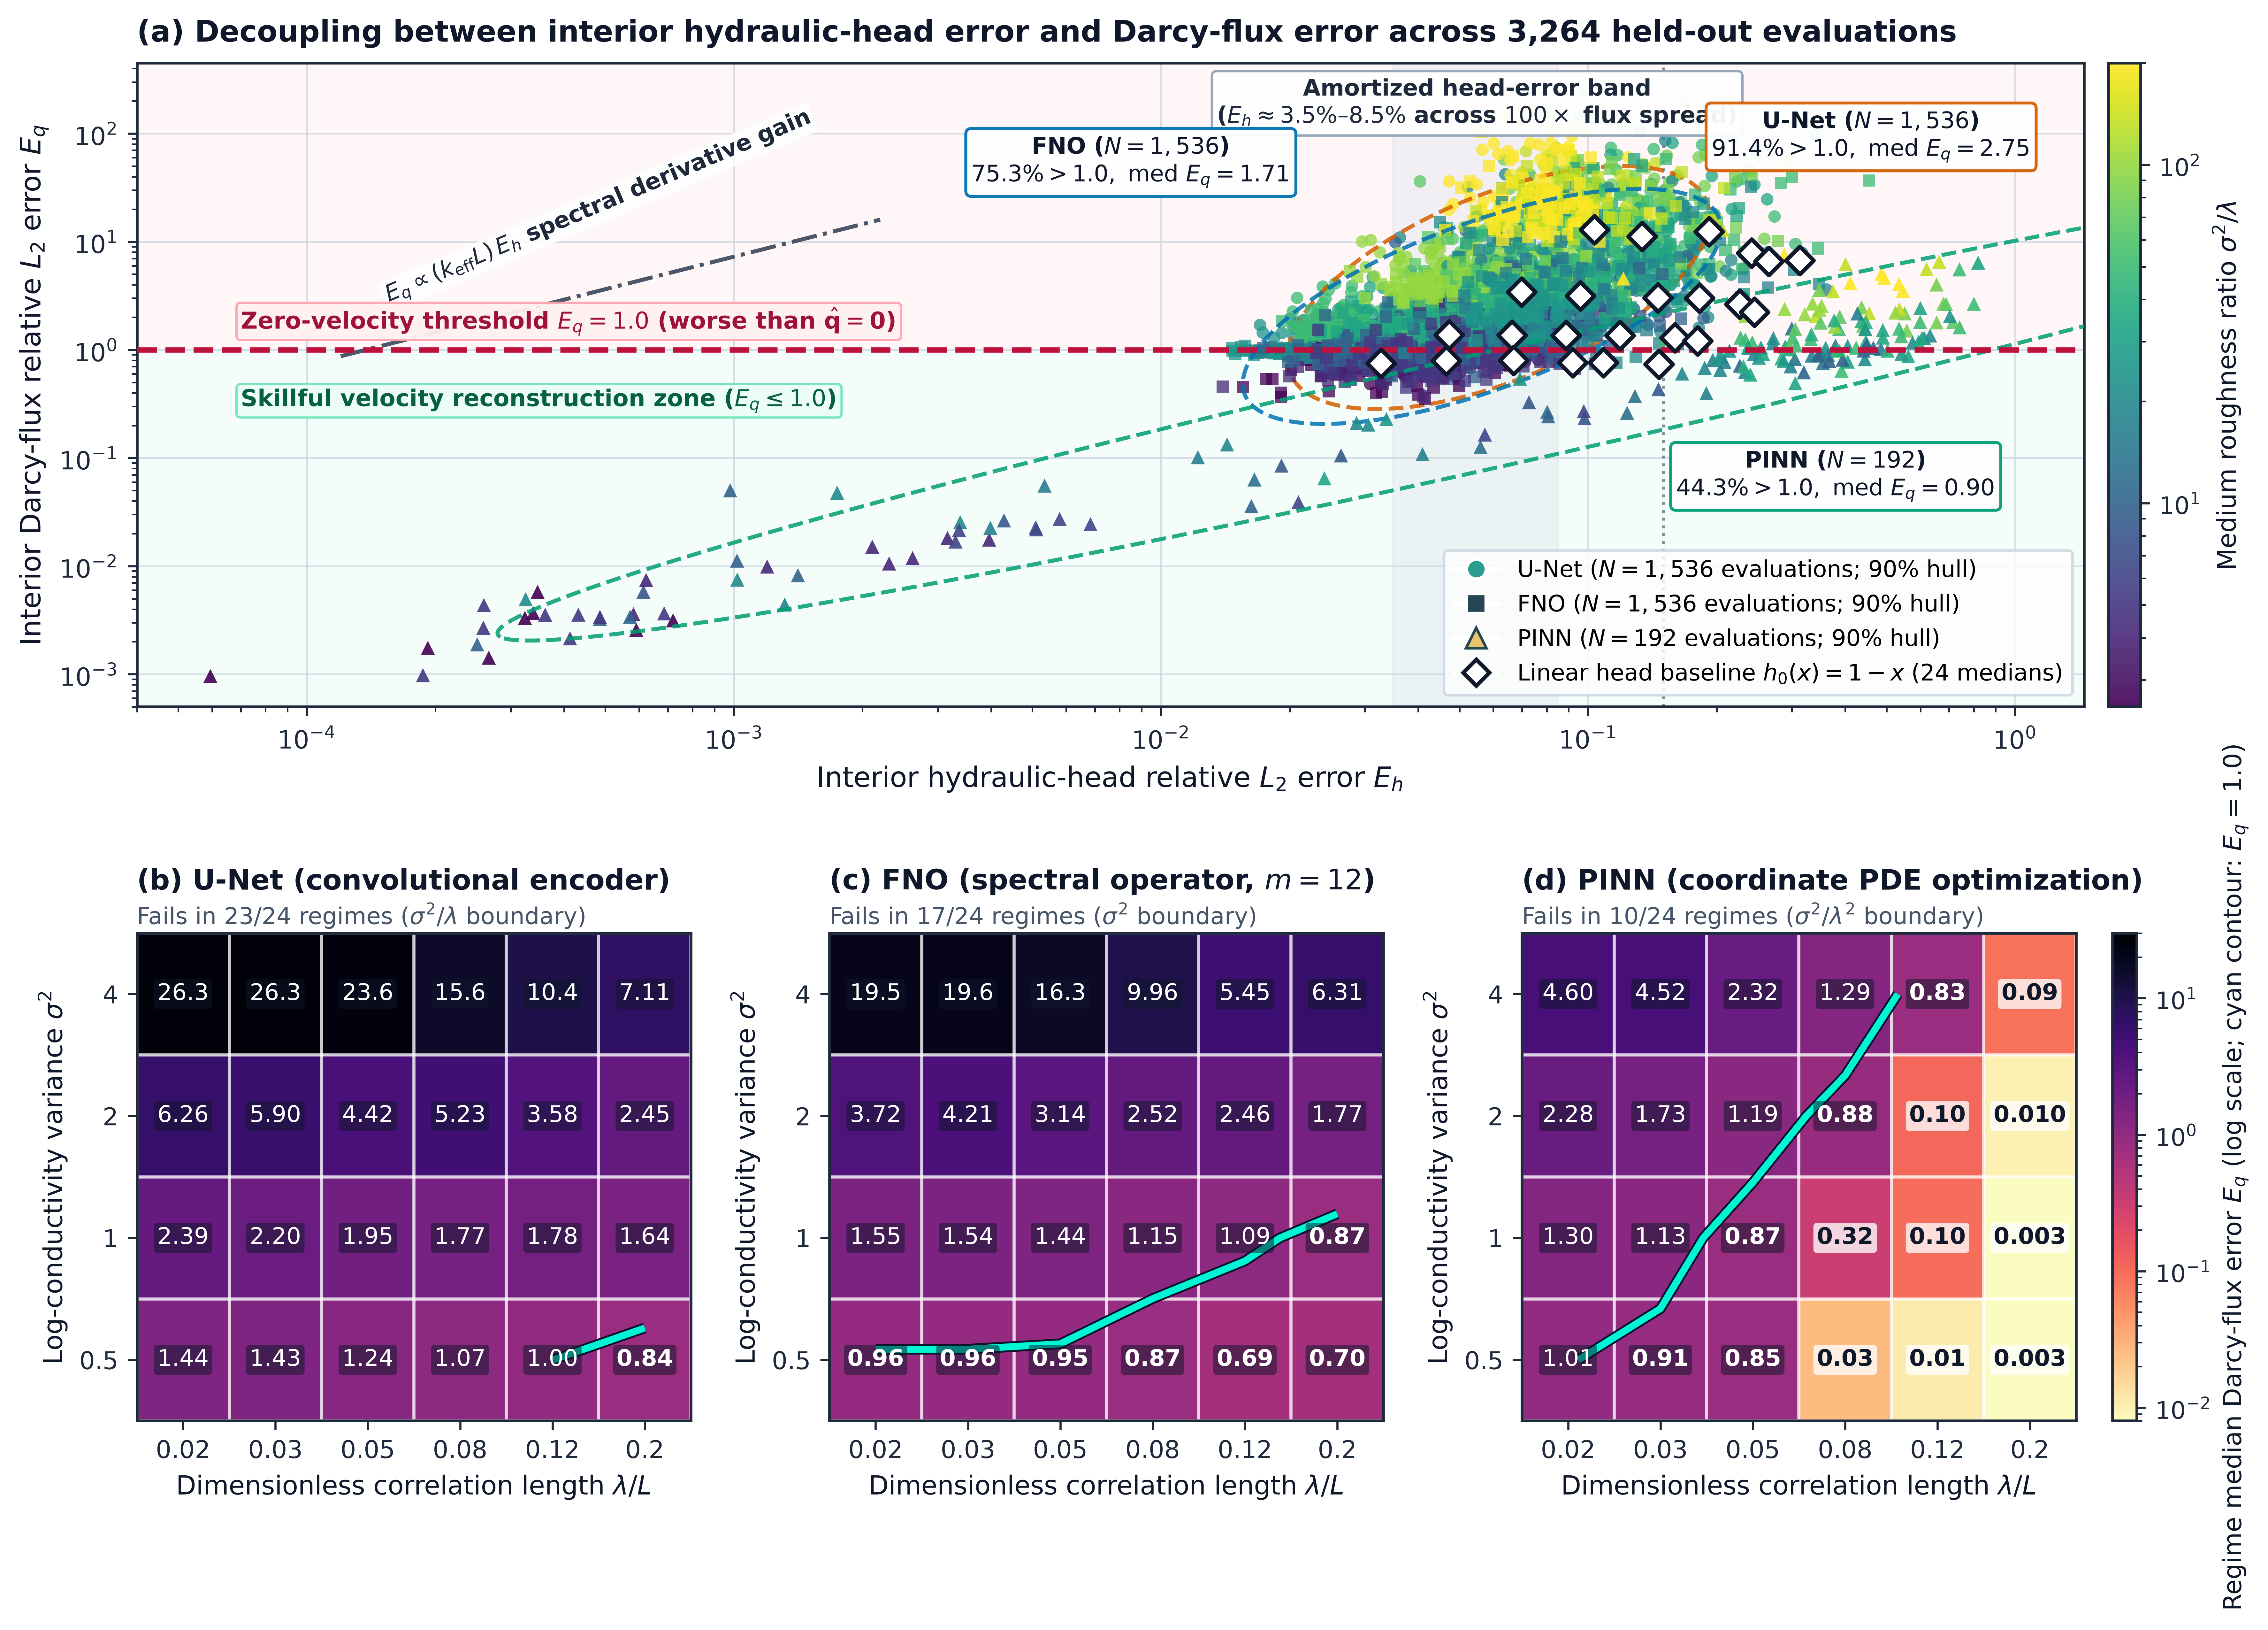
\includegraphics[width=\textwidth]{../figures/fig1_phase.png}
\caption{\textbf{The subsurface flow reliability atlas across 24 heterogeneity regimes ($3{,}264$ held-out evaluations).} \textbf{Top (a):} Instance-level hydraulic-head relative $L_2$ error ($E_h$) versus interior Darcy-flux relative $L_2$ error ($E_q$) on logarithmic axes, colored by the dimensionless roughness ratio $\sigma^2/\lambda$. Dashed ellipses show $90\%$ covariance hulls, and open white diamonds denote the untrained linear head baseline $h_0(x) = 1 - x$, which achieves lower Darcy-flux error than head-trained U-Net and FNO models across the entire short-correlation half of the atlas ($\lambda \le 0.05$). \textbf{Bottom (b--d):} Regime-median interior Darcy-flux error $E_q$ across the $(\sigma^2, \lambda)$ grid for U-Net, FNO, and PINN. The cyan contour traces the skill boundary $E_q = 1.0$.}
\label{fig:phase}
\end{figure}

Evaluating velocity accuracy on conservative TPFA face fluxes exposes a pronounced interface penalty in the baseline U-Net: its 24-regime median TPFA face-flux error reaches $5.48$ ($2.26\times$ its cell-centered median of $2.42$), producing a large divergence imbalance of $\mathcal{I}_{\text{div}} = 8.27$ because $2\Delta x$ central differences cancel period-$2\Delta x$ transposed-convolution oscillations whereas single-cell TPFA face gradients differentiate directly across them. By comparison, FNO's regime-median face-flux error is $1.67$ ($\mathcal{I}_{\text{div}} = 1.01$), and PINN achieves $0.98$ ($\mathcal{I}_{\text{div}} = 0.03$). Strikingly, across the entire short-correlation half of the atlas ($\lambda \le 0.05$), the zero-training linear profile $h_0(x) = 1 - x$ achieves lower Darcy-flux error than both head-trained U-Net and FNO surrogates (Figure~\ref{fig:phase}a). Figure~\ref{fig:anatomy} illustrates this spatial anatomy for U-Net: while predicted head contours closely match the reference ($E_h = 4.5\%$--$5.2\%$), grid-scale head residuals concentrated along high-$\nabla Y$ interfaces generate severe velocity errors ($E_q = 1.95$ and $6.23$).

\begin{figure}[t!]
\centering
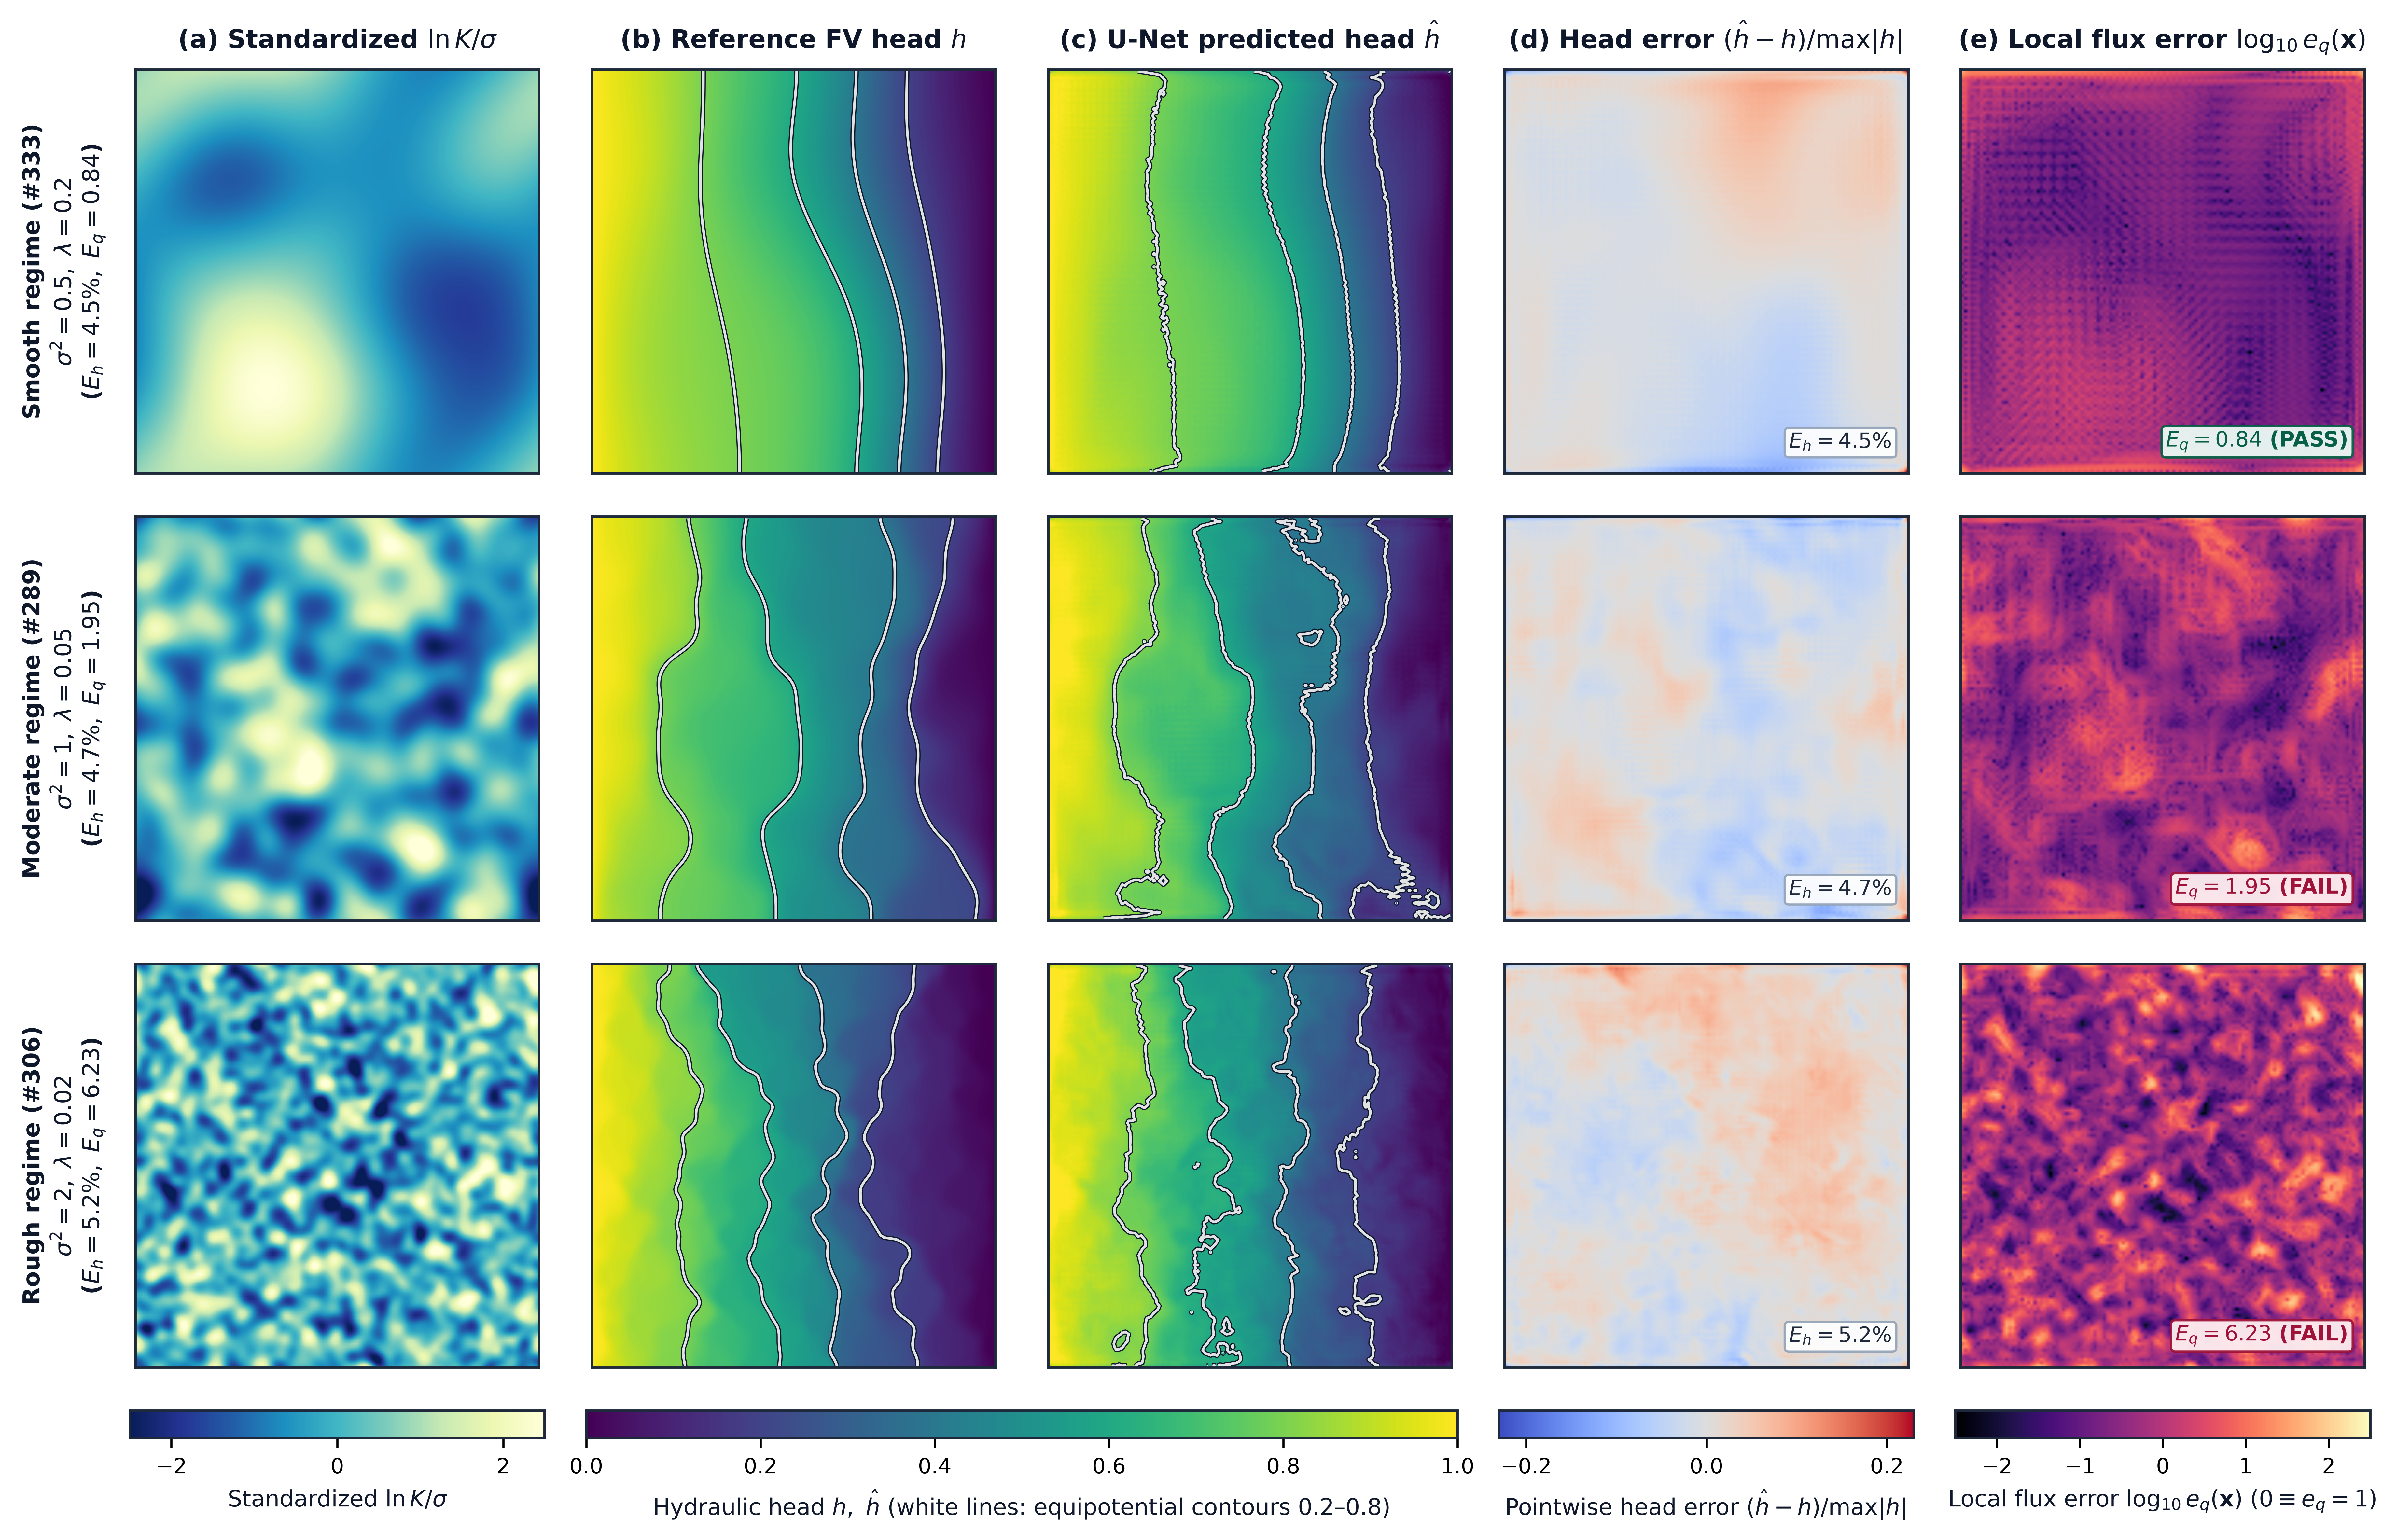
\includegraphics[width=\textwidth]{../figures/fig2_anatomy_unet.png}
\caption{\textbf{Spatial anatomy of flux blindness for the U-Net surrogate across smooth ($\sigma^2 = 0.5, \lambda = 0.20$), moderate ($\sigma^2 = 1.0, \lambda = 0.05$), and rough ($\sigma^2 = 2.0, \lambda = 0.02$) regimes.} Columns display (a) standardized log-conductivity $\ln K / \sigma$, (b) finite-volume reference head $h$, (c) U-Net predicted head $\hat{h}$, (d) normalized pointwise head error $(\hat{h} - h)/\max|h|$, and (e) logarithmic Darcy-flux error magnitude $\log_{10} e_q(\mathbf{x})$.}
\label{fig:anatomy}
\end{figure}

\subsection{Spectral Amplification Mechanism and Covariance Interventions}
\label{sec:spectral_results}

Writing $\delta h = \hat{h} - h$ for the head error and $\delta\mathbf{q} = \hat{\mathbf{q}} - \mathbf{q}$ for the Darcy velocity error under the exact conductivity field $K(\mathbf{x}) = \exp(Y(\mathbf{x}))$ yields the exact operator relation
\begin{equation}
  \delta\mathbf{q}(\mathbf{x}) = -K(\mathbf{x})\nabla\delta h(\mathbf{x}),
  \label{eq:exact_decomp}
\end{equation}
which transforms in two-dimensional Fourier space into the spectral convolution identity
\begin{equation}
  \widehat{\delta\mathbf{q}}(\mathbf{k}) = -\sum_{\mathbf{k}'} \widehat{K}(\mathbf{k} - \mathbf{k}')\,i\mathbf{k}'\,\widehat{\delta h}(\mathbf{k}').
  \label{eq:fourier_conv}
\end{equation}
Equation~\eqref{eq:fourier_conv} shows that spatial differentiation weights each head-error Fourier mode $\widehat{\delta h}(\mathbf{k}')$ by wavenumber $k' = |\mathbf{k}'|$ ($k'^2$ in energy) while convolution with $\widehat{K}$ couples errors across bandwidth $\propto 1/\lambda$. Radially averaged error spectra across smooth $(0.5, 0.20)$, moderate $(1.0, 0.05)$, and rough $(4.0, 0.02)$ regimes confirm this mechanism (Figure~\ref{fig:spectral}): relative to the reference head-fluctuation spectrum, U-Net and FNO head-error energies grow along the analytical $k^2$ slope and exceed the true signal energy by one to two orders of magnitude at $k \ge 16$. For U-Net, transposed-convolution upsampling produces a flat high-wavenumber floor across $k \in [12, 64]$; for FNO, mode truncation at $m = 12$ leaves modes $k > 12$ unattenuated; whereas PINN's error spectrum decays two to four orders of magnitude lower across $k \in [6, 64]$.

\begin{figure}[t!]
\centering
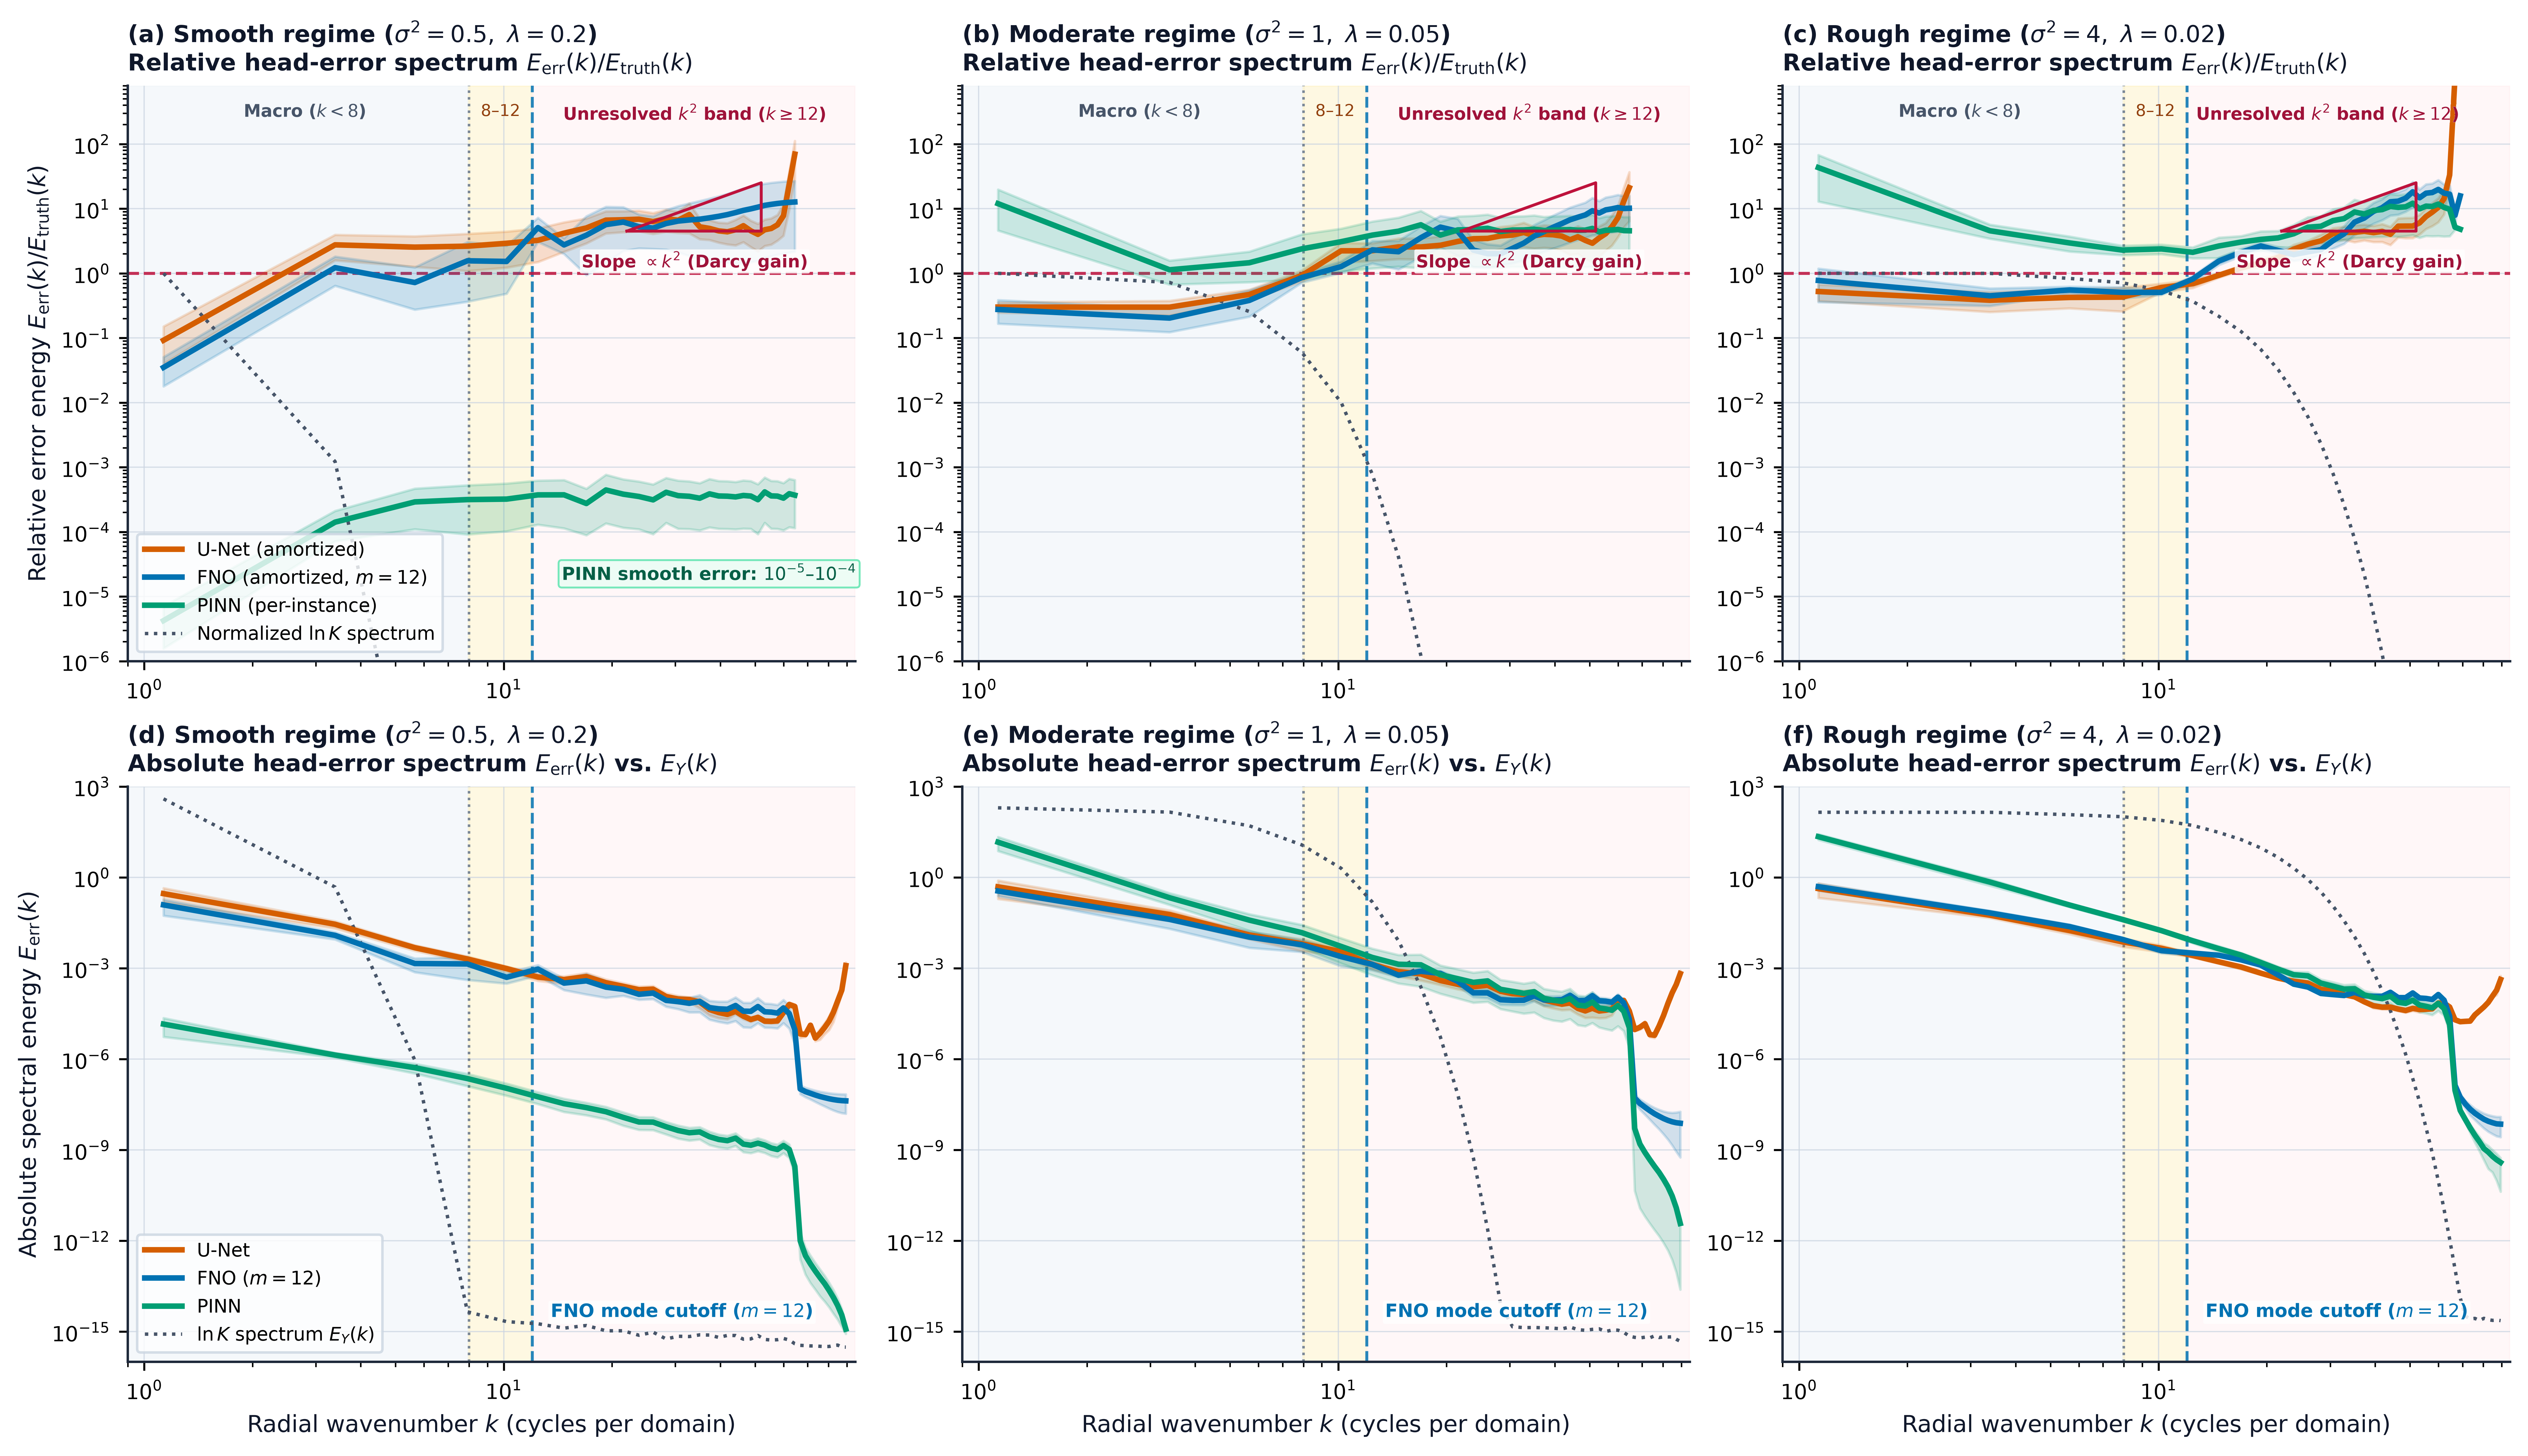
\includegraphics[width=\textwidth]{../figures/fig4_spectral.png}
\caption{\textbf{Radially averaged spectral analysis across smooth $(\sigma^2=0.5, \lambda=0.20)$, moderate $(\sigma^2=1.0, \lambda=0.05)$, and rough $(\sigma^2=4.0, \lambda=0.02)$ regimes.} \textbf{Top (a--c):} Head-error spectral energy normalized by the reference head-fluctuation spectrum ($\pm 1\text{ SD}$ ribbons), with red triangles indicating the $k^2$ derivative-gain slope. \textbf{Bottom (d--f):} Absolute head-error power spectra compared against the log-conductivity spectrum $E_Y(k)$ (dotted curve) and the FNO mode cutoff ($m = 12$).}
\label{fig:spectral}
\end{figure}

Controlled covariance-family interventions across Gaussian, Mat\'{e}rn $\nu = 3/2$, and Mat\'{e}rn $\nu = 1/2$ media at matched variance $\sigma^2$ and matched integral scale $I_Y$ confirm that small-scale roughness drives velocity error independently of $(\sigma^2, \lambda)$ (Figure~\ref{fig:covariance}). As the high-wavenumber energy fraction $\Phi(k \ge 8)$ increases from Gaussian to Mat\'{e}rn $\nu = 1/2$, median Darcy-flux error rises monotonically by $+53\%$ ($1.95 \to 2.99$) at $(1.0, 0.05)$ and $+16\%$ ($5.90 \to 6.83$) at $(2.0, 0.03)$ for U-Net, and by $+20\%$ ($1.03 \to 1.24$) and $+72\%$ ($1.91 \to 3.29$) for PINN. FNO remains nearly invariant across covariance tails ($1.44 \to 1.57$ and $4.21 \to 3.96$) because its $m = 12$ spectral truncation makes baseline FNO error primarily variance-governed. Phase-preserving Fourier shell redistribution at $(1.0, 0.05)$ and capacity ablations (expanding FNO to $m = 32$ modes or tripling U-Net parameters to $730{,}041$; Supplementary Section~S3) confirm that scaling capacity under a head-only loss yields modest $4.5\%$--$31\%$ refinements without shifting the regime failure boundary.

\begin{figure}[t!]
\centering
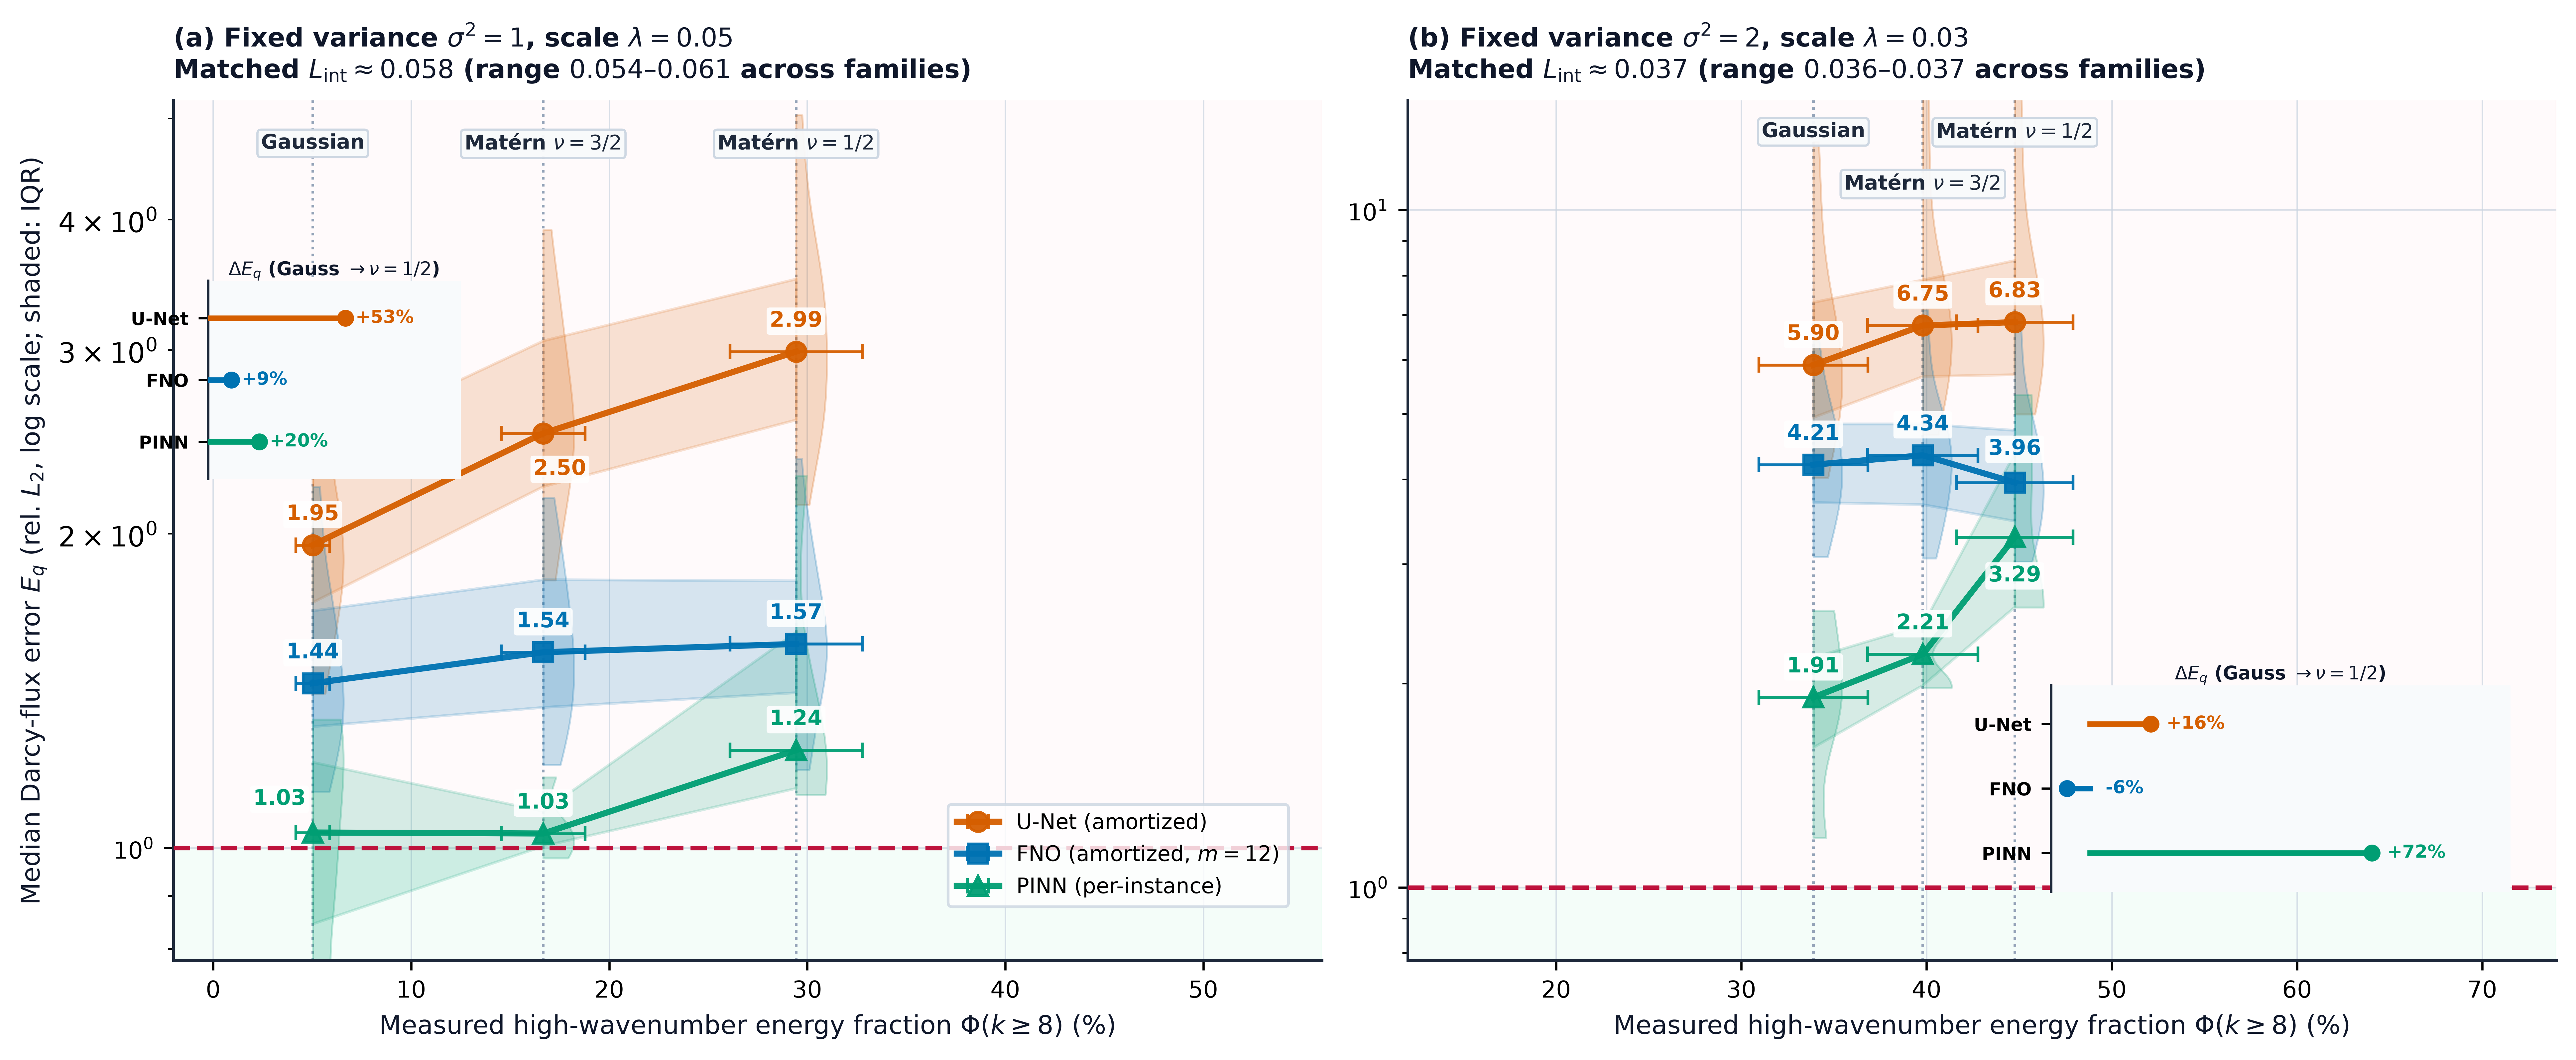
\includegraphics[width=\textwidth]{../figures/fig5_covariance.png}
\caption{\textbf{Controlled covariance-family intervention at matched variance and integral scale.} Median interior Darcy-flux error $E_q$, $25\%$--$75\%$ interquartile ribbons, and marginal density distributions plotted against the high-wavenumber spectral energy fraction $\Phi(k \ge 8)$ across Gaussian, Mat\'{e}rn $\nu = 3/2$, and Mat\'{e}rn $\nu = 1/2$ media at $(\sigma^2, \lambda) = (1.0, 0.05)$ and $(2.0, 0.03)$.}
\label{fig:covariance}
\end{figure}

\subsection{Stage 1: Pre-Training Roughness Screening Across Gaussian and Non-Gaussian Media}
\label{sec:screening_results}

Evaluating normalized head-error fields $\delta\mathbf{h}/\|\delta\mathbf{h}\|_2$ reveals that pointwise head errors are spatially phase-locked to the specific high-$\nabla Y$ interfaces of each realization, rendering error fields nearly orthogonal across realizations (mean cosine similarity $0.04$--$0.08$; Supplementary Section~S4). Consequently, transferable pre-training predictability resides in scalar roughness invariants computed directly from the conductivity ensemble $K(\mathbf{x})$. Once calibrated on the baseline benchmark archive, evaluating these descriptors on a new geological ensemble requires zero neural training or PDE solves.

Across all $3{,}264$ atlas evaluations, architecture-specific medium invariants separate reliable from failing evaluations with instance-level ROC-AUCs of $0.955$ for U-Net ($\sigma^2/\lambda$), $0.915$ for FNO ($\sigma^2$), and $0.938$ for PINN ($\sigma^2/\lambda^2$) (Table~\ref{tab:screening}). When variogram parameters $(\sigma^2, \lambda)$ are unknown, computing the parameter-free discrete gradient energy $\mathcal{R}_{\nabla Y} = L^2\langle|\nabla\ln K|^2\rangle$ directly on the grid yields nearly identical instance-level ROC-AUCs of $0.937$ (U-Net), $0.797$ (FNO), and $0.935$ (PINN). Because the baseline U-Net fails in $23/24$ atlas regimes and $11/12$ blind regimes, raw regime accuracy is confounded by class prevalence; Table~\ref{tab:screening} therefore reports sensitivity (Sens.), specificity (Spec.), false negative rate (FNR), false positive rate (FPR), and balanced accuracy ($\frac{1}{2}(\text{Sens.} + \text{Spec.})$, where a majority-class classifier scores $0.500$). Under nested leave-one-regime-out (LOO) cross-validation using Youden's $J$ statistic, the governing descriptors achieve instance-level balanced accuracies of $0.910$ (U-Net), $0.853$ (FNO), and $0.812$ (PINN).

\begin{table}[t!]
\centering
\caption{Stage~1 pre-training roughness screening across the 24-regime atlas and 12 prospective off-grid blind regimes ($64$ test realizations/regime). To account for class prevalence in baseline U-Net (23/24 atlas and 11/12 blind regimes failing), threshold-free instance ROC-AUC, sensitivity (Sens.), specificity (Spec.), false negative rate (FNR), false positive rate (FPR), and balanced accuracy (Bal.\ Acc., versus $0.500$ for a majority-class guess) are reported. Thresholds ($\sigma^2/\lambda \ge 3.33$ for U-Net, $\sigma^2 \ge 0.75$ for FNO) were frozen prior to blind testing.}
\label{tab:screening}
\resizebox{\textwidth}{!}{%
\begin{tabular}{lllllll}
\toprule
\textbf{Solver} & \textbf{Descriptor} & \textbf{Instance AUC [95\% CI]} & \textbf{LOO Bal.\ Acc.\ (Sens./Spec.)} & \textbf{Regime LOO} & \textbf{Blind Raw} & \textbf{Blind Bal.\ Acc.\ (Sens./Spec./FNR/FPR)} \\
\midrule
U-Net & $\sigma^2/\lambda$ & $0.955$ [$0.887, 0.980$] & $0.910$ ($0.90/0.92$) & $23/23$ (maj.\ $23/23$) & $12/12$ & $1.000$ ($1.00/1.00/0.00/0.00$) \\
FNO   & $\sigma^2$         & $0.915$ [$0.844, 0.953$] & $0.853$ ($0.86/0.85$) & $23/24$ (maj.\ $17/24$) & $8/12$  & $0.688$ ($1.00/0.38/0.00/0.62$) \\
PINN  & $\sigma^2/\lambda^2$ ($\mathcal{R}_{\nabla Y}$) & $0.938$ [$0.865, 0.979$] & $0.812$ ($0.82/0.80$) & $22/24$ (maj.\ $14/24$) & $2/2$   & $1.000$ ($1.00/1.00/0.00/0.00$) \\
\bottomrule
\end{tabular}%
}
\end{table}

On the 12 unseen off-grid regimes spanning interior interpolations, transition cells, and variance extrapolations up to $\sigma^2 = 6.0$ (Supplementary Table~S1), the frozen U-Net rule ($\sigma^2/\lambda \ge 3.33$) classifies all $12/12$ regimes correctly ($\text{balanced accuracy} = 1.000$, $\text{FNR} = 0.00$, $\text{FPR} = 0.00$), identifying the single reliable regime $(0.75, 0.26)$ ($E_q = 0.89$) and flagging extreme amplification at $(6.0, 0.065)$ ($E_q = 82.3$). The frozen FNO rule ($\sigma^2 \ge 0.75$) acts as a zero-false-negative safety screen ($\text{sensitivity} = 1.000$, $\text{FNR} = 0.00$ across all $8$ failing regimes), conservatively flagging borderline $\sigma^2 = 0.75$ regimes where flux-informed training is warranted. While the dimensionless invariants ($\sigma^2/\lambda, \sigma^2, \mathcal{R}_{\nabla Y}$) reflect operator structure, the numerical cutoffs are specific to the baseline architecture and training budget.

To test generalizability beyond multi-Gaussian fields, we applied the parameter-free gradient screen $\mathcal{R}_{\nabla Y}$ to the three sinuous binary-facies channelized regimes ($\sigma^2 \in \{0.5, 1.0, 2.0\}$, $16$ realizations/regime, $n = 144$ model evaluations) and the MADE-type heterogeneous alluvial lens cross-sections ($\sigma^2 = 4.5$, $16$ realizations, $n = 48$ evaluations; \texttt{src/subrel/extended\_controls.py}). Without variogram fitting, $\mathcal{R}_{\nabla Y}$ yields $354.5$, $1{,}141.4$, and $3{,}673.2$ across the three channelized regimes and $6{,}061.2$ on the MADE alluvial cross-sections, flagging sharp facies boundaries. Consistent with these high roughness values, head-trained U-Net and head-trained FNO fail in velocity ($E_q > 1.0$) across all three channelized regimes ($E_q = 1.32$--$1.43$ and $1.07$--$1.44$) and on the MADE cross-sections ($E_{q,\text{face}} = 3.34$ and $1.76$).

\subsection{Flux-Informed Operator Learning vs.\ Unsupervised Divergence Penalties}
\label{sec:repairs_results}

Before evaluating direct face-flux supervision, we benchmarked standard training modifications against matched-budget controls (Figure~\ref{fig:repairs}). While doubling the training set ($N_{\text{train}}: 128 \to 256$) stabilizes mild-variance boundary cells such as $(0.5, 0.02)$ ($E_q: 1.44 \to 0.95$ for U-Net and $0.96 \to 0.54$ for FNO) and conductivity-weighted PDE residuals cut rough-regime PINN flux error by $53\%$ at $(2.0, 0.03)$ ($1.91 \to 0.91$), unsupervised finite-volume divergence penalties exhibit a critical optimization bottleneck in rough media. Specifically, across six threshold-adjacent regimes, we compared $30$-epoch fine-tuning with an unsupervised TPFA divergence penalty ($\|\nabla_h \cdot \hat{\mathbf{q}}_f\|_2^2$, $\beta = 0.3$, analogous to recent finite-volume physics-informed neural operator losses \citep{awr2025fvfno}) against a matched-budget control continuing plain head-MSE training ($\beta = 0$) for the same $30$ epochs (Figure~\ref{fig:repairs}a). Plain MSE continuation achieves equal or lower velocity error on four of the six regimes. Mathematically, although $-\nabla\cdot(K\nabla h) = 0$ uniquely determines $h$ in the continuum limit, the discrete TPFA divergence operator $\nabla_h\cdot(T\nabla_h\hat{h})$ applies a second-order difference operator to $\hat{h}$ (whose squared $L_2$ penalty scales as $O(k^4)$ for smooth $K$ on uniform grids and becomes severely ill-conditioned across discontinuous $K$ interfaces), creating strong gradient stiffness during stochastic optimization.

\begin{figure}[t!]
\centering
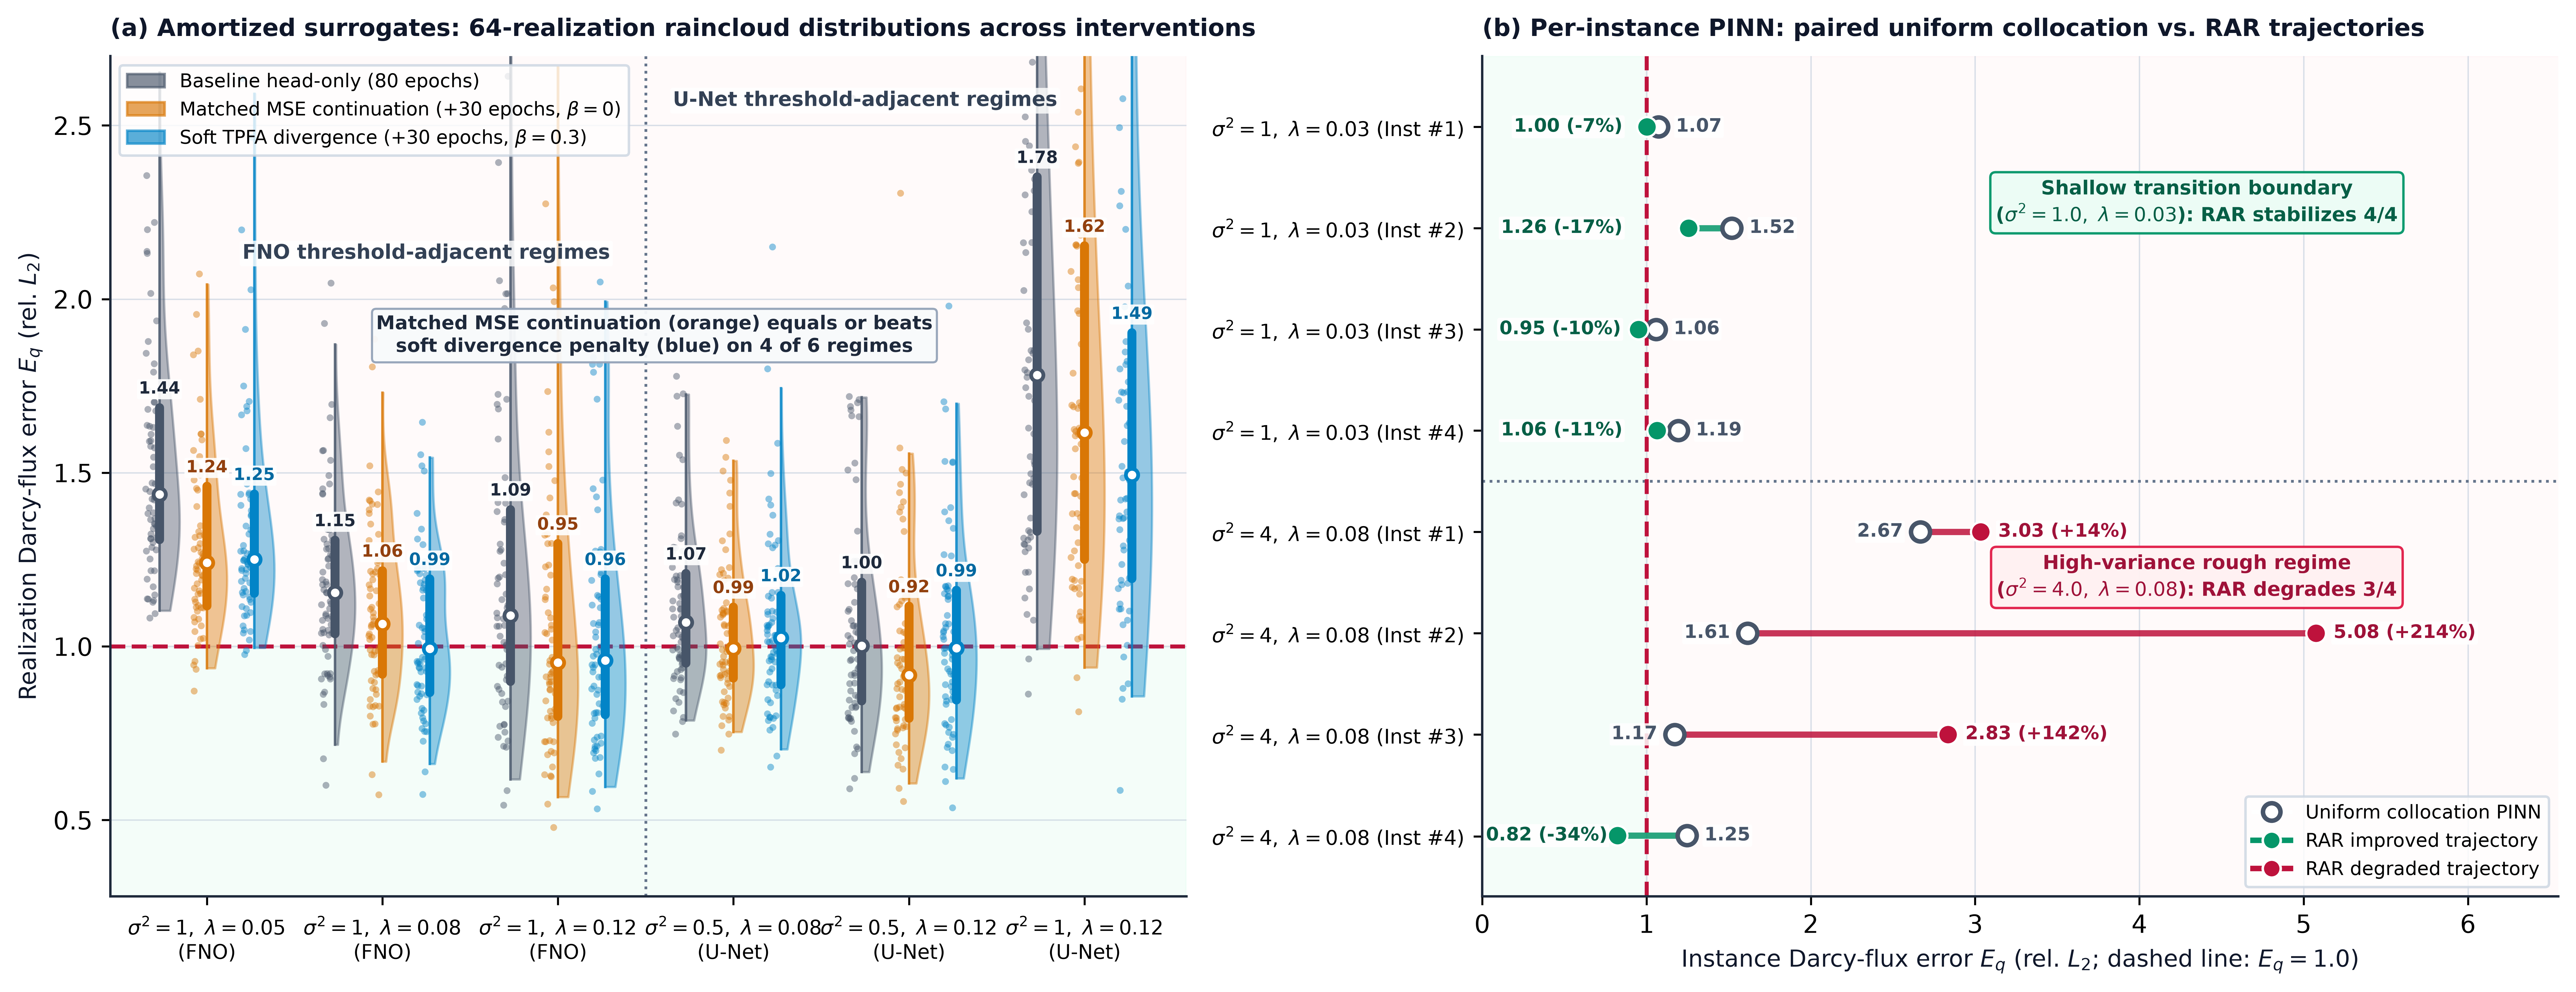
\includegraphics[width=\textwidth]{../figures/fig3_repairs.png}
\caption{\textbf{Controlled evaluation of training modifications.} \textbf{Left (a):} Across six threshold-adjacent regimes, 64-realization raincloud distributions compare the baseline model ($80$ epochs), a matched-budget MSE continuation control ($+30$ epochs, $\beta = 0$), and unsupervised TPFA divergence fine-tuning ($+30$ epochs, $\beta = 0.3$). \textbf{Right (b):} Per-instance PINN flux-error trajectories from uniform collocation to residual-adaptive resampling (RAR) at $(1.0, 0.03)$ and $(4.0, 0.08)$.}
\label{fig:repairs}
\end{figure}

By contrast, supervising the surrogate directly on reference conservative TPFA face fluxes penalizes a first-order difference in $\hat{h}$ ($O(k^2)$ energy-norm conditioning) at zero additional simulation cost:
\begin{equation}
  \mathcal{L}_{\text{total}} = \mathcal{L}_h + \frac{\alpha}{f_0}\,\frac{\|\mathbf{q}_f(\hat{h}, K) - \mathbf{q}_f(h, K)\|_{2,\Omega_{\text{int}}}^2}{\|\mathbf{q}_f(h, K)\|_{2,\Omega_{\text{int}}}^2},
  \label{eq:flux_loss}
\end{equation}
where $\alpha \in \{0.01, 0.10\}$ is normalized by the initial epoch-0 face-flux loss $f_0$. Across seven benchmark regimes ($28$ trained models under identical seeds and epoch budgets; Table~\ref{tab:flux_loss} and Figure~\ref{fig:fluxloss}), setting $\alpha = 0.01$ cuts FNO median Darcy-flux error by $52\%$--$73\%$, while $\alpha = 0.10$ cuts FNO median flux error by $63\%$--$95\%$ (moving five of seven regimes below $E_q = 1.0$ and reducing $(2.0, 0.03)$ and $(4.0, 0.02)$ from $4.21$ and $19.55$ to $1.03$ and $1.04$). Crucially, evaluating the $\alpha = 0.01$ Flux-FNO zero-shot on non-Gaussian media cuts median face-flux error by $68\%$--$73\%$ across all three sinuous channelized regimes ($E_{q,\text{face}} = 0.35, 0.34, 0.40 \le 1.0$) and by $58\%$ on the MADE-type alluvial lens cross-sections ($E_{q,\text{face}}: 1.76 \to 0.74 \le 1.0$).

\begin{table}[t!]
\centering
\caption{Effect of conservative TPFA face-flux supervision (Eq.~\eqref{eq:flux_loss}) on regime-median interior Darcy-flux error $E_q$ across seven Gaussian regimes ($n = 64$ test realizations/regime) and zero-shot generalization to non-Gaussian sinuous channelized ($n = 16$ realizations/regime) and MADE-type alluvial lens ($n = 16$ realizations) media. Bold values satisfy $E_q \le 1.0$.}
\label{tab:flux_loss}
\resizebox{\textwidth}{!}{%
\begin{tabular}{lcccccc}
\toprule
\textbf{Regime $(\sigma^2, \lambda)$ or Facies Type} & \textbf{FNO $\alpha=0$} & \textbf{FNO $\alpha=0.01$} & \textbf{FNO $\alpha=0.10$} & \textbf{U-Net $\alpha=0$} & \textbf{U-Net $\alpha=0.01$} & \textbf{U-Net $\alpha=0.10$} \\
\midrule
$(0.5, 0.20)$ Smooth Gaussian      & \textbf{0.70} & \textbf{0.32} ($-53\%$) & \textbf{0.20} ($-71\%$) & \textbf{0.84} & \textbf{0.79} ($-6\%$) & 1.04 ($+24\%$) \\
$(0.5, 0.08)$ Mild Gaussian        & \textbf{0.87} & \textbf{0.31} ($-65\%$) & \textbf{0.19} ($-78\%$) & 1.07 & 1.01 ($-6\%$) & 1.07 ($0\%$) \\
$(1.0, 0.12)$ Moderate $\lambda$   & 1.09 & \textbf{0.47} ($-56\%$) & \textbf{0.30} ($-73\%$) & 1.78 & 1.71 ($-4\%$) & 1.94 ($+9\%$) \\
$(1.0, 0.05)$ Transition Gaussian  & 1.44 & \textbf{0.51} ($-64\%$) & \textbf{0.38} ($-73\%$) & 1.95 & 1.88 ($-3\%$) & 2.12 ($+9\%$) \\
$(2.0, 0.08)$ Moderate $\sigma^2$  & 2.52 & 1.20 ($-52\%$) & \textbf{0.93} ($-63\%$) & 5.23 & 5.27 ($+1\%$) & 4.57 ($-13\%$) \\
$(2.0, 0.03)$ Rough Gaussian       & 4.21 & 1.45 ($-65\%$) & 1.03 ($-76\%$) & 5.90 & 5.53 ($-6\%$) & 4.74 ($-20\%$) \\
$(4.0, 0.02)$ Extreme Gaussian     & 19.55 & 5.24 ($-73\%$) & 1.04 ($-95\%$) & 26.34 & 25.14 ($-5\%$) & 20.56 ($-22\%$) \\
\midrule
Sinuous Channelized ($\sigma^2=2.0$, $n=16$) & 1.44 & \textbf{0.42} ($-71\%$) & --- & 1.43 & --- & --- \\
MADE Alluvial Lenses ($\sigma^2=4.5$, $n=16$) & 1.75 & \textbf{0.75} ($-57\%$) & --- & 1.93 & --- & --- \\
\bottomrule
\end{tabular}%
}
\end{table}

\begin{figure}[t!]
\centering
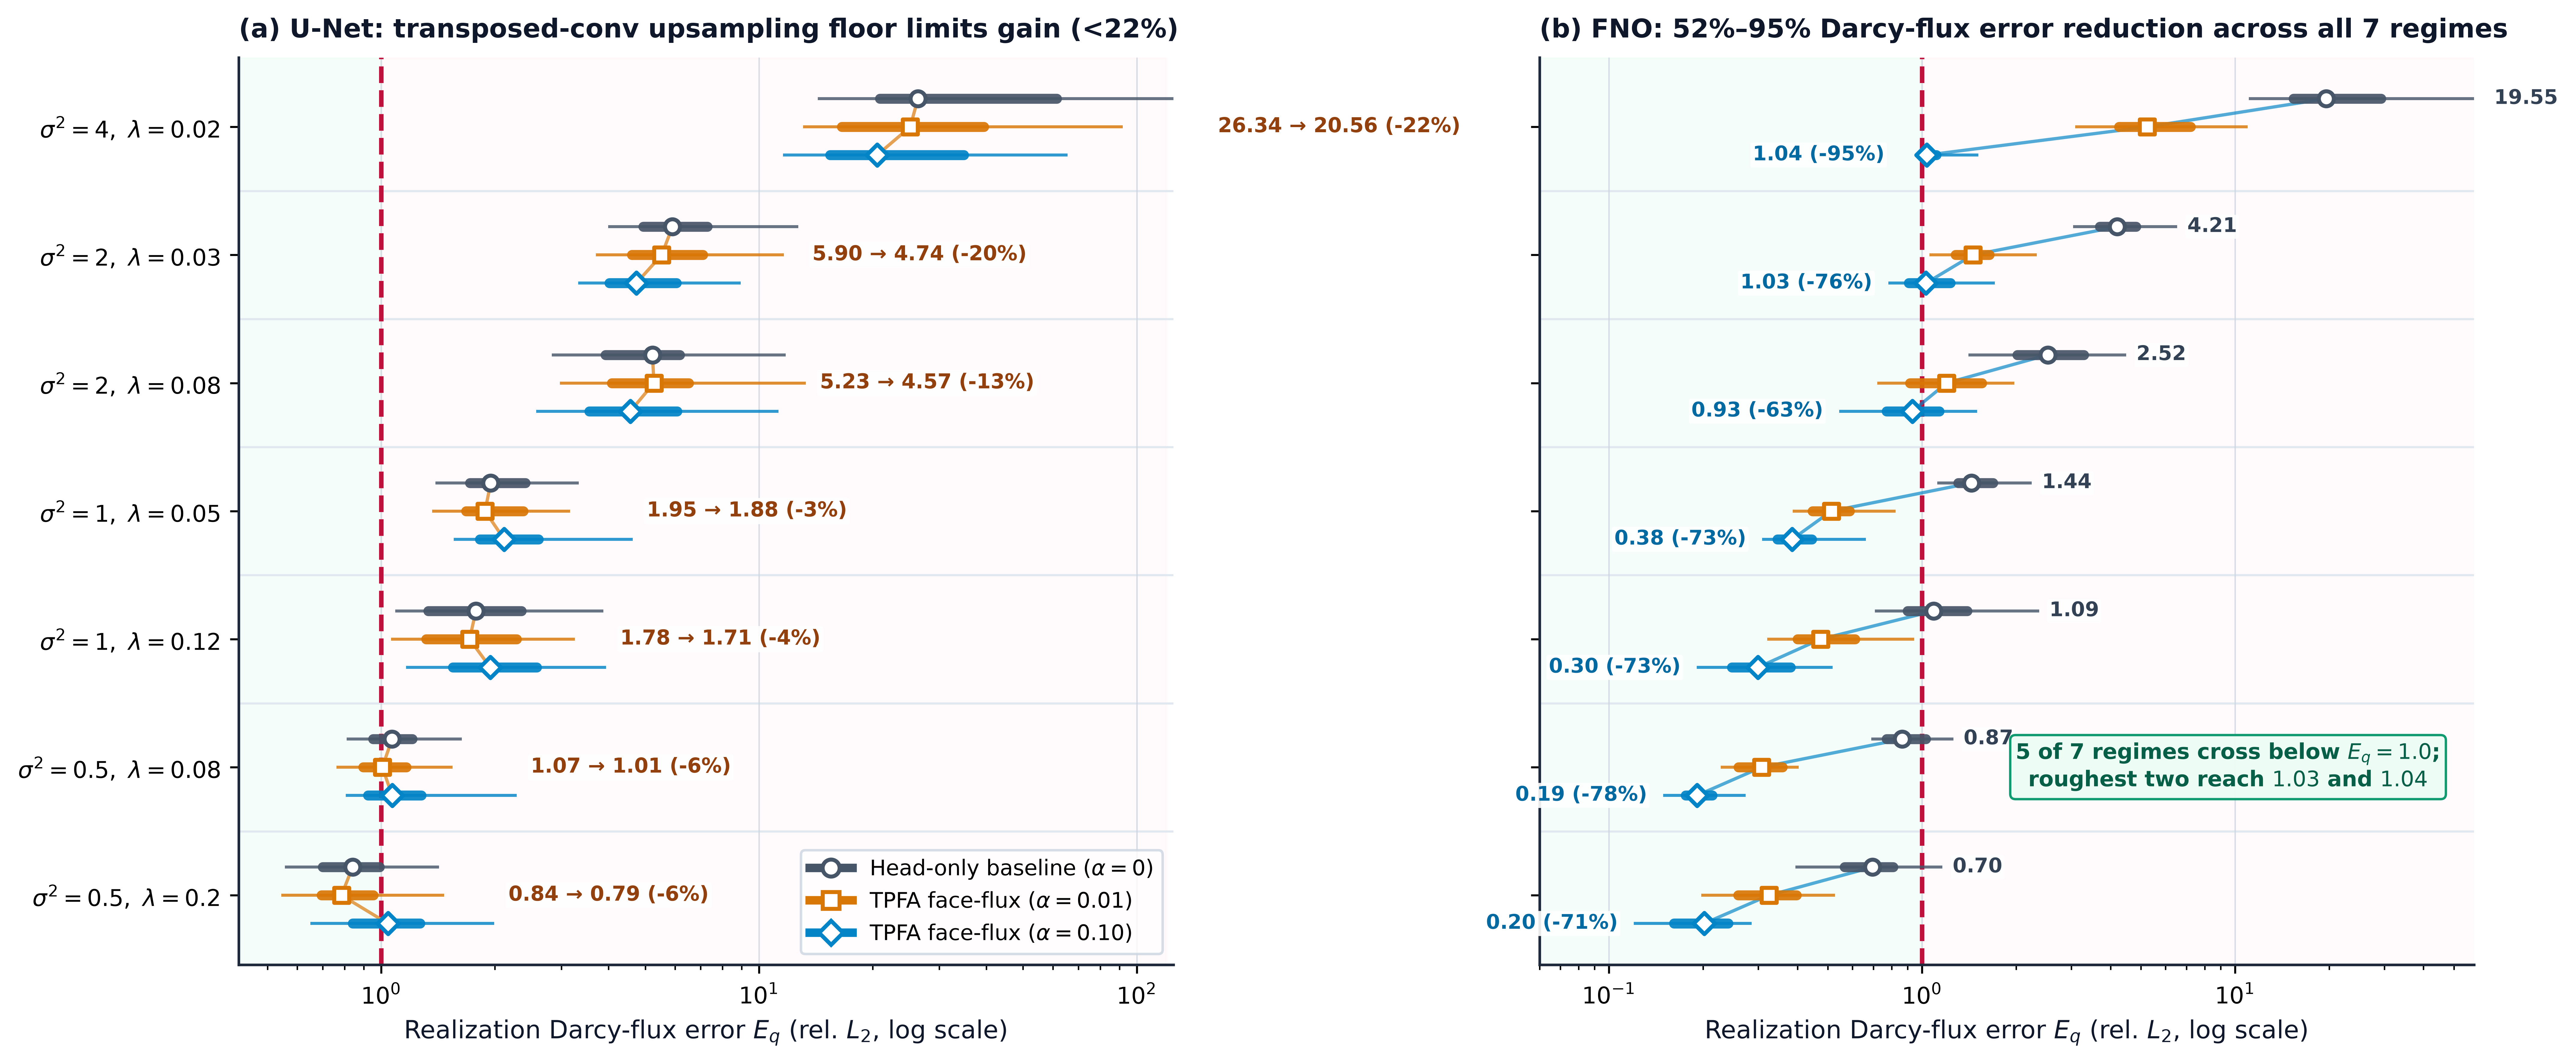
\includegraphics[width=\textwidth]{../figures/fig6_fluxloss.png}
\caption{\textbf{Architectural response to conservative TPFA face-flux supervision across seven benchmark regimes.} Horizontal quantile forest plots ($25\%$--$75\%$ IQR capsules, $5\%$--$95\%$ whiskers, and medians across $\alpha \in \{0, 0.01, 0.10\}$) for \textbf{(a)} U-Net and \textbf{(b)} FNO. FNO cuts median velocity error by $52\%$--$73\%$ at $\alpha = 0.01$ and $63\%$--$95\%$ at $\alpha = 0.10$, whereas baseline U-Net is limited by stride-2 transposed-convolution interface oscillations.}
\label{fig:fluxloss}
\end{figure}

In contrast to FNO, the baseline U-Net changes by only $-22\%$ to $+24\%$ under Eq.~\eqref{eq:flux_loss}. In our controlled decoder ablation (\texttt{ResizeUNet}), replacing stride-2 transposed convolutions with bilinear upsampling and $3 \times 3$ convolution collapses U-Net's TPFA face-to-cell-center error ratio from $1.96\times$ to $1.05\times$ at $(1.0, 0.05)$ and from $1.65\times$ to $1.08\times$ at $(2.0, 0.03)$, cutting divergence imbalance $\mathcal{I}_{\text{div}}$ by $78\%$ ($5.32 \to 1.19$) and $73\%$ ($13.09 \to 3.54$). Under $\alpha = 0.01$ at $(2.0, 0.03)$, \texttt{ResizeUNet} reduces face-flux error by $22\%$ ($5.54 \to 4.30$) compared with $-6\%$ for the transposed-convolution baseline, confirming that transposed convolutions drive the interface amplification while FNO's global spectral modes provide stronger long-range derivative coupling ($-65\%$).

\subsection{Two-Level Transport Decoupling and Stage 2 Hybrid Multigrid Recovery}
\label{sec:transport_results}

Pollock streamline tracking across $24$ test realizations ($984$ particles per solver; Table~\ref{tab:transport} and Figure~\ref{fig:transport}) reveals a two-level physical decoupling between state accuracy, global $L_2$ flux accuracy, and local mass conservation. At the first level, head-trained U-Net ($E_h = 5.1\%$) and head-trained FNO ($E_h = 5.2\%$) suffer near-total streamline breakdown: $0.0\%$ ($0/984$) and $2.2\%$ ($22/984$) of released particles reach the outflow boundary, while $73.9\%$ and $89.4\%$ stall inside artificial interior divergence sinks. At the second level, supervising FNO on TPFA face fluxes ($\alpha = 0.01$) cuts median face-flux error from $1.49$ to $0.52$ and raises particle breakthrough more than $24$-fold to $54.4\%$ ($535/984$ particles across $20/24$ realizations) with an accurate median paired travel-time ratio of $t / t_{\text{ref}} = 1.04$. Nevertheless, residual local divergence ($\mathcal{I}_{\text{div}} = 0.23$) in the roughest realizations still traps $17.8\%$ of trajectories and backwashes $27.8\%$, demonstrating that global $L_2$ velocity skill ($E_q < 1.0$), while necessary for accurate travel times, does not guarantee $100\%$ streamline connectivity without pointwise divergence closure ($\nabla_h \cdot \mathbf{q}_f = 0$). Conversely, the untrained linear profile $h_0(x) = 1 - x$ achieves $100\%$ arrival because $\partial_y h_0 \equiv 0$ eliminates interior sinks, but its 1D row locking across low-$K$ inclusions yields a large flux error ($E_{q,\text{face}} = 1.27$) and a $1.33\times$ slow bias in travel time.

\begin{table}[t!]
\centering
\caption{Pollock advective particle-tracking outcomes and initial-guess comparison across $24$ held-out test realizations ($984$ particles per velocity source) spanning $(\sigma^2, \lambda) \in \{(0.5, 0.08), (1.0, 0.05), (2.0, 0.03)\}$, before and after Stage~2 single-cycle AMG defect correction ($\hat{h}_{\text{corr}} = \hat{h} + z_1$).}
\label{tab:transport}
\resizebox{\textwidth}{!}{%
\begin{tabular}{lcccccc}
\toprule
\textbf{Velocity Field Source ($24$ cells, $984$ particles)} & \textbf{Med.\ $E_{q,\text{face}}$} & \textbf{Arrived (\%)} & \textbf{Stalled (\%)} & \textbf{Backwashed (\%)} & \textbf{Active Cells} & \textbf{Med.\ $t / t_{\text{ref}}$ [Note]} \\
\midrule
Finite-volume reference ($h_{\text{ref}}$) & $0.000$ & 984 (100.0\%) & 0 (0.0\%) & 0 (0.0\%) & $24 / 24$ & $1.00$ [exact] \\
Untrained linear profile ($h_0 = 1 - x$)   & $1.272$ & 984 (100.0\%) & 0 (0.0\%) & 0 (0.0\%) & $24 / 24$ & $1.33$ [$1.06$--$2.72$] \\
U-Net (head-only, $\alpha = 0$)            & $3.358$ & 0 (0.0\%)     & 727 (73.9\%) & 257 (26.1\%) & $0 / 24$ & Undefined \\
FNO (head-only, $\alpha = 0$)              & $1.487$ & 22 (2.2\%)    & 880 (89.4\%) & 82 (8.3\%)   & $1 / 24$ & $2.42$ [$1$ cell] \\
FNO (flux-weighted, $\alpha = 0.01$)       & $0.519$ & 535 (54.4\%)  & 175 (17.8\%) & 274 (27.8\%) & $20 / 24$ & $1.04$ [$0.90$--$3.79$] \\
\midrule
Zero guess ($h = 0$) + 1 AMG V-cycle       & $0.349$ & 123 (12.5\%)  & 482 (49.0\%) & 379 (38.5\%) & $14 / 24$ & $1.05$ [incomplete] \\
Linear profile ($h_0$) + 1 AMG V-cycle     & $0.190$ & 984 (100.0\%) & 0 (0.0\%)    & 0 (0.0\%)    & $24 / 24$ & $1.00$ [$2.4\times$ err.] \\
U-Net ($\alpha = 0$) + 1 AMG V-cycle       & $0.226$ & 725 (73.7\%)  & 259 (26.3\%) & 0 (0.0\%)    & $24 / 24$ & $1.03$ [$0$ backwash] \\
FNO ($\alpha = 0$) + 1 AMG V-cycle         & $0.166$ & 827 (84.0\%)  & 140 (14.2\%) & 17 (1.7\%)   & $24 / 24$ & $1.00$ [$1.0026$] \\
\textbf{FNO ($\alpha = 0.01$) + 1 AMG V-cycle} & $\mathbf{0.080}$ & \textbf{925 (94.0\%)} & \textbf{51 (5.2\%)} & \textbf{8 (0.8\%)} & $\mathbf{24 / 24}$ & $\mathbf{1.00}$ [$\mathbf{0.9982}$] \\
\bottomrule
\end{tabular}%
}
\end{table}

\begin{figure}[t!]
\centering
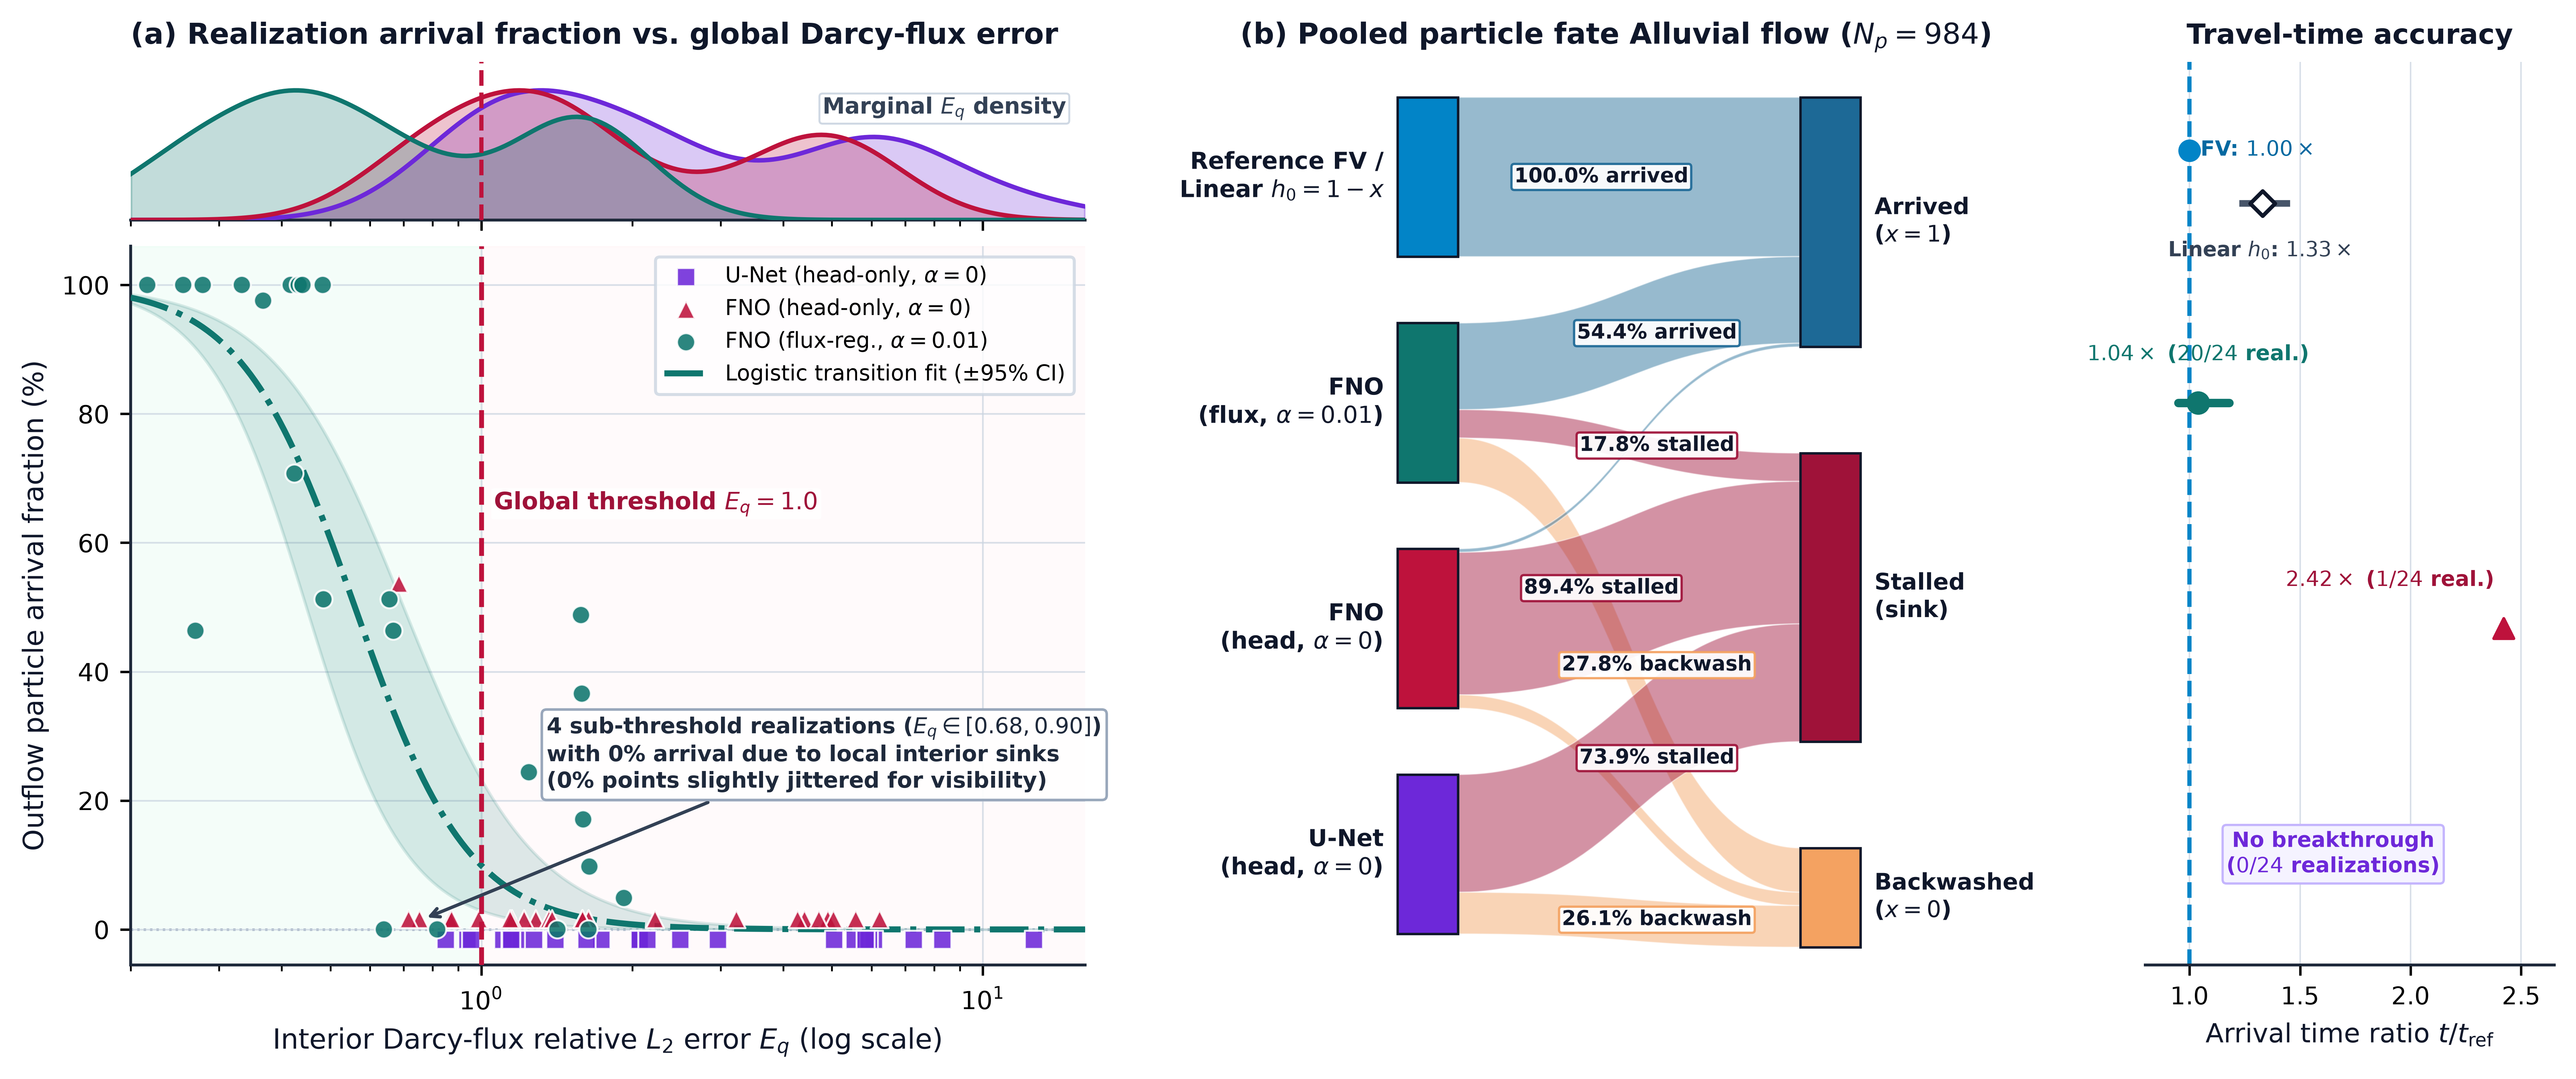
\includegraphics[width=\textwidth]{../figures/fig7_transport.png}
\caption{\textbf{Advective particle-tracking fates and travel-time accuracy ($984$ particles across $24$ realizations).} \textbf{Left (a):} Outflow arrival percentage plotted against interior Darcy-flux error $E_q$. \textbf{Right (b):} Alluvial diagram tracing particle fates into outflow arrival, interior stalling, or inflow backwashing, paired with arrival travel-time ratios $t / t_{\text{ref}}$.}
\label{fig:transport}
\end{figure}

\subsection{Stage 2: Reference-Free AMG Residual Screening, Defect Correction, and Cost--Accuracy Scaling}
\label{sec:posterior_results}

To screen and correct individual velocity predictions online without ground-truth solves, we exploit the exact discrete dual energy identity for the TPFA residual $r = b - A_K \hat{h}$ and true head error $e = h - \hat{h}$ \citep{vohralik2008,ern2010posteriori,ernst2026cert}:
\begin{equation}
  A_K e = r, \qquad \|\delta\mathbf{F}\|_{T^{-1}}^2 = \delta\mathbf{F}^\top T^{-1}\delta\mathbf{F} = e^\top A_K e = r^\top A_K^{-1} r,
  \label{eq:posterior_identity}
\end{equation}
where $T$ is the diagonal matrix of harmonic face transmissibilities. Approximating $z_1 \approx A_K^{-1} r$ via a single smoothed-aggregation AMG V-cycle \citep{notay2010agg,pyamg2023} yields the protected reference-free residual indicator
\begin{equation}
  \eta_F = \frac{\|\mathbf{q}_f(z_1)\|_{2,\Omega_{\text{int}}}}{\max\!\big(\|\mathbf{q}_f(\hat{h})\|_{2,\Omega_{\text{int}}},\,\epsilon\big)}, \quad \epsilon = 10^{-12},
  \label{eq:eta_f}
\end{equation}
and the one-step defect-corrected head field $\hat{h}_{\text{corr}} = \hat{h} + z_1$.

Across all $3{,}264$ atlas evaluations, $\eta_F$ ranks true interior face-flux error with Spearman $\rho = 0.92$ and separates failed ($E_{q,\text{face}} > 1.0$) from reliable predictions with $\text{ROC-AUC} = 0.997$, substantially outperforming the unpreconditioned residual $\|r\|_2/\|b\|_2$ ($\rho = 0.66$, dropping to $\rho = 0.47$ on FNO). The same indicator achieves $\text{ROC-AUC} = 0.9998$ (95\% bootstrap CI $[0.9985, 1.0000]$, $n = 144$ across $3$ regimes $\times 16$ realizations $\times 3$ models) on the sinuous channelized regimes, $\text{ROC-AUC} = 0.9912$ (95\% CI $[0.9676, 1.0000]$, $n = 48$ across $16$ realizations $\times 3$ models) on the MADE alluvial cross-sections, and $\text{ROC-AUC} = 1.0000$ (95\% CI $[1.0000, 1.0000]$, $\rho = 0.955$, $n = 54$) when evaluating trained U-Net, head-FNO, and Flux-FNO models directly on refined $256 \times 256$ conductivity fields.

Applying $z_1$ as a single-step defect correction ($\hat{h}_{\text{corr}} = \hat{h} + z_1$) cuts pooled median face-flux error by $93\%$ across the $128^2$ Gaussian atlas ($2.83 \to 0.20$), by $90.3\%$ on channelized media ($1.18 \to 0.115$), by $88.5\%$ on real $256^2$ neural predictions ($2.04 \to 0.235$), and restores Pollock particle arrival on the MADE alluvial cross-sections from $26.2\%$ to $89.3\%$ ($E_{q,\text{face}}: 0.74 \to 0.139$). Crucially, Table~\ref{tab:transport} demonstrates that the neural operator provides genuine warm-start value: after one AMG V-cycle, `Flux-FNO + 1 V-cycle` achieves median $E_h = 0.56\%$ and $E_{q,\text{face}} = 0.080$ ($94.0\%$ Pollock arrival across $24/24$ realizations, $0.8\%$ backwashing, travel-time ratio $1.00$), which is $2.4\times$ more accurate in face flux than `Linear + 1 V-cycle` ($E_{q,\text{face}} = 0.190$) and $4.4\times$ more accurate than `Zero + 1 V-cycle` ($E_{q,\text{face}} = 0.349$, $12.5\%$ arrival). Standalone AMG starting from $h = 0$ or $h_0(x) = 1 - x$ requires $2.0$ V-cycles (double the multigrid solve work) to match the flux accuracy of `Flux-FNO + 1 V-cycle`.

Evaluating end-to-end computational costs clarifies the operational break-even regimes between standalone Flux-FNO, hybrid `Flux-FNO + 1-cycle AMG`, and direct numerical solvers. Training Flux-FNO requires $T_{\text{train}} \approx 110\text{ s}$ on $128$ realizations. In moderate heterogeneity ($\sigma^2 \le 1.0$) or channelized media where standalone Flux-FNO achieves $E_q = 0.31$--$0.51$ without multigrid post-processing, a single neural forward pass takes $T_{\text{neural}} = 2.8\text{ ms}$ ($128^2$) or $33\text{ ms}$ ($256^2$) versus $T_{\text{direct}} = 41\text{ ms}$ ($128^2$) or $133\text{ ms}$ ($256^2$), amortizing training after $\sim 2{,}800$ forward evaluations (a single ensemble data-assimilation workflow). When strict local conservation is required for streamline tracking on refined grids, $T_{\text{neural}} + T_{\text{AMG setup}} + T_{\text{V-cycle}}$ requires $0.080\text{ s}$ versus $0.133\text{ s}$ for direct factorization on real $256^2$ predictions ($1.66\times$ speedup; $3.6\times$ speedup when the AMG hierarchy is reused across boundary conditions, and $3.2\times$ total speedup on $512^2$ grids at $0.42\text{ s}$ versus $1.34\text{ s}$).

\section{Discussion}
\label{sec:discussion}

Our findings resolve why subsurface neural surrogates with test head errors below $5\%$--$6\%$ and head $R^2 > 0.99$ frequently fail in downstream mass-balance or solute-transport modeling \citep{fuks2020limits,wang2020tgnn,massbal2024}. Standard $L_2$ head training weights all Fourier modes equally ($|\widehat{\delta h}(\mathbf{k})|^2$), whereas the Darcy velocity norm weights modes by $k^2 |\widehat{\delta h}(\mathbf{k})|^2$ convolved with $\widehat{K}(\mathbf{k})$. In rough media, $L_2$-trained surrogates fit the dominant macro-scale pressure ramp ($k \le 4$) while leaving a flat high-wavenumber residual floor ($k \ge 12$) that accounts for $<1\%$ of head variance but reverses local cell-face gradients and traps $73.9\%$--$89.4\%$ of advective particles. Subsurface surrogate benchmarks should therefore report conservative TPFA face-flux error ($E_{q,\text{face}}$), local divergence imbalance ($\mathcal{I}_{\text{div}}$), and Pollock breakthrough statistics benchmarked against the zero-training linear profile $h_0(x) = 1 - x$.

Comparing solver architectures and training objectives highlights the interplay between operator parametrization and numerical conditioning. Whereas unsupervised finite-volume divergence losses \citep{awr2025fvfno} penalize a second-order difference operator ($\nabla_h\cdot(T\nabla_h\hat{h})$) that is ill-conditioned across high-wavenumber modes and discontinuous $K$ interfaces ($\sigma^2 \ge 1.0$), direct supervision on reference TPFA face fluxes constrains a first-order difference in $\hat{h}$ ($H^1_K$ energy norm) using global FNO modes, reducing velocity error by $52\%$--$95\%$ across Gaussian regimes and by $57\%$--$73\%$ zero-shot on channelized and MADE-type alluvial media. In convolutional U-Nets, replacing stride-2 transposed convolutions with bilinear resize-convolution eliminates the $2.26\times$ TPFA interface error amplification, although global spectral layers remain superior to local $3 \times 3$ stencils for capturing long-range flux coupling.

Synthesizing these components yields the two-stage operational workflow summarized in Table~\ref{tab:algorithm_workflow}. In Stage~1, practitioners evaluate $\sigma^2/\lambda$, $\sigma^2$, or parameter-free discrete gradient energy $\mathcal{R}_{\nabla Y}$ directly on the target conductivity ensemble to route rough regimes to conservative face-flux training. In Stage~2, online inference uses standalone Flux-FNO for fast ensemble flux estimation or pairs Flux-FNO with a single $O(N^2)$ AMG V-cycle ($\eta_F$ screening and $\hat{h} + z_1$ defect correction) to guarantee local mass conservation and domain-spanning streamline transport. While validated here on two-dimensional steady-state single-phase flow across Gaussian, channelized, and alluvial lens media, the discrete TPFA face-flux loss and dual-norm AMG residual identity ($A_K e = r$) extend directly to three-dimensional hexahedral grids and implicit time-stepping schemes in transient or multiphase porous media flow.

\begin{table}[t!]
\centering
\caption{Executable two-stage computational workflow (\texttt{SubsurfaceReliability v1.0}) for pre-training roughness screening, flux-informed operator training, and online AMG residual screening and defect correction.}
\label{tab:algorithm_workflow}
\footnotesize
\begin{tabular}{p{3.2cm}p{12.4cm}}
\toprule
\textbf{Workflow Stage} & \textbf{Algorithmic Procedure and Operational Decision Rules} \\
\midrule
\textbf{Inputs} & Discretized log-conductivity ensemble $\{Y^{(m)}(\mathbf{x})\}_{m=1}^M$ on $N \times N$ grid ($K = \exp Y$); target solver family $\mathcal{M} \in \{\text{U-Net}, \text{FNO}, \text{PINN}\}$; conservative TPFA stencil $A_K \mathbf{h} = \mathbf{b}$. \\
\midrule
\textbf{Stage 1: Pre-Training Roughness Screening \& Loss Selection} & \textbf{1a. Compute medium roughness invariant ($O(N^2)$ per field):} Evaluate $(\sigma^2, \lambda)$ or parameter-free discrete gradient energy $\mathcal{R}_{\nabla Y} = L^2 \langle |\nabla Y|^2 \rangle$. \newline \textbf{1b. Apply calibrated regime safety screen:} Compare against baseline thresholds: $\sigma^2/\lambda < 3.33$ (U-Net), $\sigma^2 < 0.75$ (FNO), or $\sigma^2/\lambda^2 < 200$ / $\mathcal{R}_{\nabla Y} < 400$ (PINN; recalibratable via Youden's $J$). \newline \textbf{1c. Select training objective:} If flagged as rough ($\ge$ threshold), train FNO with conservative TPFA face-flux supervision $\mathcal{L}(\theta) = \mathcal{L}_h + (\alpha / f_0)\mathcal{L}_q$ ($\alpha \in [0.01, 0.10]$) or solve PINN with conductivity-normalized/weighted residuals. \\
\midrule
\textbf{Stage 2: Online AMG Screening \& Defect Correction} & \textbf{2a. Fast neural forward pass:} Predict hydraulic head $\hat{h}$ ($2.8\text{ ms}$ at $128^2$, $33\text{ ms}$ at $256^2$); use standalone Flux-FNO directly for ensemble flux estimation when $\sigma^2 \le 1.0$. \newline \textbf{2b. Single-cycle AMG dual-norm indicator ($O(N^2)$):} For rough media or transport workflows, assemble $r = b - A_K \hat{h}$, compute one AMG V-cycle $z_1 \approx A_K^{-1} r$, and evaluate $\eta_F = \|\mathbf{q}_f(z_1)\|_{2,\Omega_{\text{int}}} / \max(\|\mathbf{q}_f(\hat{h})\|_{2,\Omega_{\text{int}}}, 10^{-12})$. \newline \textbf{2c. Reference-free screening and 1-step correction:} If $\eta_F$ exceeds tolerance, apply $\hat{h}_{\text{corr}} = \hat{h} + z_1$ and reconstruct conservative face fluxes $\mathbf{q}_f(\hat{h}_{\text{corr}})$ (cutting flux error by $89\%$--$93\%$ and restoring $89\%$--$94\%$ streamline arrival). \\
\bottomrule
\end{tabular}
\end{table}

\section{Conclusions}
\label{sec:conclusions}

We have developed and validated a reliability-aware two-stage computational workflow (\texttt{SubsurfaceReliability v1.0}) across 24 lognormal heterogeneity regimes ($3{,}264$ evaluations), 12 unseen off-grid regimes, and non-Gaussian channelized and MADE-type alluvial lens media. Head-trained U-Net and FNO surrogates achieve median head errors of $5.9\%$ and $5.5\%$ yet exceed the zero-velocity error threshold ($E_q > 1.0$) in $91.4\%$ and $75.3\%$ of evaluations because $k^2$ derivative weighting amplifies high-wavenumber head residuals across conductivity interfaces, while stride-2 transposed convolutions induce a $2.26\times$ TPFA interface error amplification in U-Net that is eliminated by bilinear resize-convolution ($1.03\times$ to $1.08\times$). Prior to training, medium roughness invariants ($\sigma^2/\lambda$, $\sigma^2$, and parameter-free discrete gradient energy $\mathcal{R}_{\nabla Y}$) screen regime suitability with instance-level ROC-AUCs of $0.915$--$0.955$, achieving $1.000$ balanced accuracy ($12/12$) for U-Net and $100\%$ sensitivity for FNO on 12 unseen off-grid regimes. Direct supervision on conservative TPFA face fluxes ($\alpha \in \{0.01, 0.10\}$) overcomes the ill-conditioning of second-order unsupervised divergence penalties, reducing FNO velocity error by $52\%$--$95\%$ across Gaussian regimes and by $57\%$--$73\%$ zero-shot on channelized and MADE-type alluvial lens media. Finally, a single AMG V-cycle provides a reference-free residual indicator $\eta_F$ ($\text{ROC-AUC} = 0.991$--$1.000$ across Gaussian, channelized, alluvial, and $256^2$ grids), cuts median face-flux error by $89\%$--$93\%$ as a one-step defect correction ($2.4\times$ to $4.4\times$ more accurate than one AMG cycle from linear or zero guesses), and restores $94.0\%$ Pollock streamline breakthrough with a median travel-time ratio of $1.00$.

\section{Computer Code and Data Availability}
\label{sec:data}

\begin{itemize}
  \item \textbf{Name of code / software:} \texttt{SubsurfaceReliability} (Version 1.0)
  \item \textbf{Developer:} Zijie Deng (Jiangxi Provincial Key Laboratory of Water Resources Allocation and Efficient Utilization, Jiangxi University of Water Resources and Electric Power; email: \texttt{3335196397vip@gmail.com})
  \item \textbf{Year first available:} 2026
  \item \textbf{Program language:} Python 3.12 (with Bash automation scripts)
  \item \textbf{Software required:} NumPy ($\ge 2.0$), SciPy ($\ge 1.14$), PyTorch ($\ge 2.4$), PyAMG ($\ge 5.2$), pandas ($\ge 2.2$), Matplotlib ($\ge 3.9$), scikit-learn ($\ge 1.5$), and h5py ($\ge 3.11$); locked environment specifications are recorded in \texttt{environment.txt}
  \item \textbf{Licensing provisions:} MIT Open-Source License
  \item \textbf{Repository, model weights, and user documentation:} The complete source code, user guide (\texttt{USER\_GUIDE.md}), quickstart tutorial (\texttt{tutorials/quickstart\_workflow.py}), unit tests, archived evaluation records (\texttt{runs/} and \texttt{data/}), and all $409$ trained PyTorch model checkpoints (\texttt{SubsurfaceReliability\_v1.0\_model\_weights.tar.gz} via GitHub Releases) are openly available at \url{https://github.com/yuelangmanle/SubsurfaceReliability}. Running \texttt{bash scripts/reproduce\_figures\_and\_tables.sh} executes the four-gate numerical verification suite, runs the unit tests, prints all summary tables, and reproduces Figures~1--7 in approximately $15\text{ s}$ on a standard desktop CPU.
\end{itemize}

\section*{CRediT Authorship Contribution Statement}
\textbf{Zijie Deng:} Conceptualization, Methodology, Software, Validation, Formal analysis, Investigation, Data curation, Visualization, Writing -- original draft, Writing -- review \& editing. \textbf{Zhenyu Liao:} Data curation, Validation, Writing -- review \& editing. \textbf{Jiyang Yu:} Investigation, Visualization, Writing -- review \& editing.

\section*{Declaration of Competing Interest}
The authors declare that they have no known competing financial interests or personal relationships that could have appeared to influence the work reported in this paper.

\section*{Acknowledgments}
This research did not receive any specific grant from funding agencies in the public, commercial, or not-for-profit sectors.

\begin{thebibliography}{99}

\bibitem[Alhubail et al.(2024)]{alhubail2024weight}
Alhubail, A., Fahs, M., Lehmann, F., Hoteit, H., 2024. Modeling fluid flow in heterogeneous porous media with physics-informed neural networks: Weighting strategies for the mixed pressure head-velocity formulation. Adv. Water Resour. 193, 104797.

\bibitem[Bandai and Ghezzehei(2021)]{bandai2021wrr}
Bandai, H., Ghezzehei, T.A., 2021. Physics-informed neural networks with monotonicity constraints for Richardson--Richards equation: Estimation of observation retention and permeability curve parameters. Water Resour. Res. 57 (2), e2020WR027642.

\bibitem[Bear(1972)]{bear1972dynamics}
Bear, J., 1972. Dynamics of Fluids in Porous Media. Elsevier, New York.

\bibitem[Bell et al.(2023)]{pyamg2023}
Bell, W.N., Olson, L.N., Schroder, J.B., Southworth, B.S., 2023. PyAMG: Algebraic multigrid solvers in Python. J. Open Source Softw. 8 (87), 5495.

\bibitem[Blunt(2017)]{blunt2017multiphase}
Blunt, M.J., 2017. Multiphase Flow in Permeable Media: A Pore-Scale Perspective. Cambridge University Press, Cambridge.

\bibitem[Carrera et al.(2005)]{carrera2005inverse}
Carrera, J., Alcolea, A., Medina, A., Hidalgo, J., Slooten, L.J., 2005. Inverse problem in hydrogeology. Hydrogeol. J. 13 (1), 206--222.

\bibitem[Chang and Zhang(2020)]{chang2020dl}
Chang, H., Zhang, D., 2020. Machine learning subsurface flow equations from data. Comput. Geosci. 24 (3), 839--854.

\bibitem[Chen and Oliver(2013)]{chen2013ensemble}
Chen, Y., Oliver, D.S., 2013. Levenberg--Marquardt forms of the iterative ensemble smoother for efficient history matching and uncertainty quantification. Comput. Geosci. 17 (4), 689--703.

\bibitem[Cuomo et al.(2022)]{cuomo2022scientific}
Cuomo, S., Di Cola, V.S., Giampaolo, F., Rozza, G., Raissi, M., Piccialli, F., 2022. Scientific machine learning through physics-informed neural networks: Where we are and what's next. J. Sci. Comput. 92 (3), 88.

\bibitem[Dagan(1989)]{dagan1989flow}
Dagan, G., 1989. Flow and Transport in Porous Formations. Springer-Verlag, Berlin.

\bibitem[Delhomme(1979)]{delhomme1979spatial}
Delhomme, J.P., 1979. Spatial variability and uncertainty in groundwater flow parameters: A geostatistical approach. Water Resour. Res. 15 (2), 269--280.

\bibitem[Dietrich and Newsam(1993)]{dietrich1993fast}
Dietrich, C.R., Newsam, G.N., 1993. A fast and exact method for multidimensional Gaussian stochastic simulations. Water Resour. Res. 29 (8), 2861--2869.

\bibitem[E and Yu(2018)]{weinan2018drm}
E, W., Yu, B., 2018. The Deep Ritz Method: A deep learning-based numerical algorithm for solving variational problems. Commun. Math. Stat. 6 (1), 1--12.

\bibitem[Efendiev et al.(2013)]{efendiev2013gmsfem}
Efendiev, Y., Galvis, J., Hou, T.Y., 2013. Generalized multiscale finite element methods (GMsFEM). J. Comput. Phys. 251, 116--135.

\bibitem[Emerick and Reynolds(2013)]{emerick2013esmda}
Emerick, A.A., Reynolds, A.C., 2013. Ensemble smoother with multiple data assimilation. Comput. Geosci. 55, 3--15.

\bibitem[Ern et al.(2010)]{ern2010posteriori}
Ern, A., Stephansen, A.F., Vohral\'{\i}k, J., 2010. Guaranteed and robust discontinuous Galerkin a posteriori error estimates for convection--diffusion--reaction problems. J. Comput. Appl. Math. 234 (1), 114--130.

\bibitem[Ernst et al.(2025)]{ernst2026cert}
Ernst, L., Rekatsinas, N., Urban, K., 2025. A posteriori certification of PDE approximations with particular application to neural networks. Preprint, arXiv:2502.20336.

\bibitem[Eymard et al.(2000)]{eymard2000}
Eymard, R., Gallou\"{e}t, T., Herbin, R., 2000. Finite volume methods. In: Ciarlet, P.G., Lions, J.L. (Eds.), Handbook of Numerical Analysis, Vol. 7. North-Holland, Amsterdam, pp. 713--1020.

\bibitem[Fuks and Tchelepi(2020)]{fuks2020limits}
Fuks, O., Tchelepi, H.A., 2020. Limitations of physics-informed machine learning for nonlinear two-phase transport in porous media. J. Mach. Learn. Model. Comput. 1 (1), 19--37.

\bibitem[Gelhar(1993)]{gelhar1993stochastic}
Gelhar, L.W., 1993. Stochastic Subsurface Hydrology. Prentice-Hall, Englewood Cliffs, NJ.

\bibitem[Grossmann et al.(2024)]{grossmann2024fem}
Grossmann, T.G., Komorowska, U.J., Latz, J., Sch\"{o}nlieb, C.-B., 2024. Can physics-informed neural networks beat the finite element method? IMA J. Appl. Math. 89 (1), 143--174.

\bibitem[Jagtap et al.(2020)]{jagtap2020cpinn}
Jagtap, A.D., Kharazmi, E., Karniadakis, G.E., 2020. Conservative physics-informed neural networks on discrete domains for conservation laws: Applications to forward and inverse problems. Comput. Methods Appl. Mech. Eng. 365, 113028.

\bibitem[Karniadakis et al.(2021)]{karniadakis2021piml}
Karniadakis, G.E., Kevrekidis, I.G., Lu, L., Perdikaris, P., Wang, S., Yang, L., 2021. Physics-informed machine learning. Nat. Rev. Phys. 3 (6), 422--440.

\bibitem[Karumuri et al.(2020)]{karumuri2020simfree}
Karumuri, S., Tripathy, R., Bilionis, I., Panchal, J., 2020. Simulator-free solution of high-dimensional stochastic elliptic partial differential equations using deep neural networks. J. Comput. Phys. 404, 109120.

\bibitem[Kashefi and Mukerji(2022)]{kashefi2023pnet}
Kashefi, A., Mukerji, T., 2022. Physics-informed PointNet: A deep learning solver for steady-state advection--dispersion equations to conduct flow and transport simulations in discrete fracture networks. J. Comput. Phys. 468, 111510.

\bibitem[Khazal et al.(2025)]{awr2026benchmark}
Khazal, H., Singh, S., Singh, N., Abass, K., Partonia, S., 2025. Physics-informed neural operators and generative models for multi-task surrogate modeling of CO2 plume migration in ultra-heterogeneous reservoirs: A benchmark comparative study. Adv. Water Resour., in press.

\bibitem[Kitanidis and Lee(2014)]{kitanidis2014pcga}
Kitanidis, P.K., Lee, J., 2014. Principal Component Geostatistical Approach for large-dimensional inverse problems. Water Resour. Res. 50 (7), 5428--5443.

\bibitem[Kovachki et al.(2023)]{kovachki2023no}
Kovachki, N., Li, Z., Liu, B., Azizzadenesheli, K., Bhattacharya, K., Stuart, A., Anandkumar, A., 2023. Neural operator: Learning maps between function spaces with applications to PDEs. J. Mach. Learn. Res. 24 (89), 1--97.

\bibitem[Krishnapriyan et al.(2021)]{krishnapriyan2021}
Krishnapriyan, A., Gholami, A., Zhe, S., Kirby, R., Mahoney, M.W., 2021. Characterizing possible failure modes in physics-informed neural networks. In: Advances in Neural Information Processing Systems (NeurIPS), Vol. 34, pp. 26548--26560.

\bibitem[Laloy and Vrugt(2012)]{laloy2012dream}
Laloy, E., Vrugt, J.A., 2012. High-dimensional posterior exploration of hydrologic models using multiple-try DREAM(ZS) and high-performance computing. Water Resour. Res. 48 (1), W01526.

\bibitem[Lauzon(2024)]{lauzon2024unet}
Lauzon, D., 2024. A U-Net architecture as a surrogate model combined with a geostatistical spectral algorithm for transient groundwater flow inverse problems. Adv. Water Resour. 189, 104726.

\bibitem[Li et al.(2021)]{li2021fno}
Li, Z., Kovachki, N., Azizzadenesheli, K., Liu, B., Bhattacharya, K., Stuart, A., Anandkumar, A., 2021. Fourier neural operator for parametric partial differential equations. In: International Conference on Learning Representations (ICLR).

\bibitem[Lie(2019)]{lie2019mrst}
Lie, K.-A., 2019. An Introduction to Reservoir Simulation Using MATLAB/GNU Octave: User Guide for the MATLAB Reservoir Simulation Toolbox (MRST). Cambridge University Press, Cambridge.

\bibitem[Lu et al.(2021a)]{lu2021deeponet}
Lu, L., Jin, P., Pang, G., Zhang, Z., Karniadakis, G.E., 2021a. Learning nonlinear operators via DeepONet based on the universal approximation theorem of operators. Nat. Mach. Intell. 3 (3), 218--229.

\bibitem[Lu et al.(2021b)]{lu2021deepxde}
Lu, L., Meng, X., Mao, Z., Karniadakis, G.E., 2021b. DeepXDE: A deep learning library for solving differential equations. SIAM Rev. 63 (1), 208--228.

\bibitem[Lu et al.(2021c)]{lu2021pinn}
Lu, L., Pestourie, R., Yao, W., Wang, Z., Verdugo, F., Johnson, S.G., 2021c. Physics-informed neural networks with hard constraints for inverse design. SIAM J. Sci. Comput. 43 (6), B1105--B1132.

\bibitem[Lu et al.(2022)]{lu2022comprehensive}
Lu, L., Meng, X., Cai, S., Mao, Z., Goswami, S., Zhang, Z., Karniadakis, G.E., 2022. A comprehensive and fair comparison of two neural operators (with practical extensions) based on FAIR data. Comput. Methods Appl. Mech. Eng. 393, 114778.

\bibitem[Mamud et al.(2024)]{massbal2024}
Mamud, M.L., Mudunuru, M.K., Karra, S., Ahmmed, B., 2024. Quantifying local and global mass balance errors in physics-informed neural networks. Sci. Rep. 14, 15541.

\bibitem[Mo et al.(2019)]{mo2019deep}
Mo, S., Zhu, Y., Zabaras, N., Shi, X., Wu, J., 2019. Deep convolutional encoder-decoder networks for uncertainty quantification of dynamic multiphase flow in heterogeneous media. Water Resour. Res. 55 (1), 703--728.

\bibitem[Notay(2010)]{notay2010agg}
Notay, Y., 2010. An aggregation-based algebraic multigrid method. Electron. Trans. Numer. Anal. 37, 123--146.

\bibitem[Pollock(1988)]{pollock1988}
Pollock, D.W., 1988. Semianalytical computation of path lines for finite-difference models. Ground Water 26 (6), 743--750.

\bibitem[Rahaman et al.(2019)]{rahaman2019bias}
Rahaman, N., Baratin, A., Arpit, D., Draxler, F., Lin, M., Hamprecht, F., Bengio, Y., Courville, A., 2019. On the spectral bias of neural networks. In: International Conference on Machine Learning (ICML), PMLR 97, pp. 5301--5310.

\bibitem[Raissi et al.(2019)]{raissi2019pinn}
Raissi, M., Perdikaris, P., Karniadakis, G.E., 2019. Physics-informed neural networks: A deep learning framework for solving forward and inverse problems involving nonlinear partial differential equations. J. Comput. Phys. 378, 686--707.

\bibitem[Raviart and Thomas(1977)]{raviart1977mixed}
Raviart, P.-A., Thomas, J.M., 1977. A mixed finite element method for 2-nd order elliptic problems. In: Galligani, I., Magenes, E. (Eds.), Mathematical Aspects of Finite Element Methods, Lecture Notes in Mathematics, Vol. 606. Springer, Berlin, pp. 292--315.

\bibitem[Roache(1998)]{roache1998}
Roache, P.J., 1998. Verification and Validation in Computational Science and Engineering. Hermosa Publishers, Albuquerque, NM.

\bibitem[Ronneberger et al.(2015)]{ronneberger2015unet}
Ronneberger, O., Fischer, P., Brox, T., 2015. U-Net: Convolutional networks for biomedical image segmentation. In: Medical Image Computing and Computer-Assisted Intervention (MICCAI), LNCS 9351, pp. 234--241.

\bibitem[Rubin(2003)]{rubin2003applied}
Rubin, Y., 2003. Applied Stochastic Hydrogeology. Oxford University Press, New York.

\bibitem[Sirignano and Spiliopoulos(2018)]{sirignano2018dgm}
Sirignano, J., Spiliopoulos, K., 2018. DGM: A deep learning algorithm for solving partial differential equations. J. Comput. Phys. 375, 1339--1364.

\bibitem[Tang et al.(2020)]{tang2020dl}
Tang, M., Liu, Y., Durlofsky, L.J., 2020. A deep-learning-based surrogate model for data assimilation in dynamic subsurface flow problems. J. Comput. Phys. 413, 109456.

\bibitem[Tartakovsky et al.(2020)]{tartakovsky2020physics}
Tartakovsky, A.M., Marrero, C.O., Perdikaris, P., Tartakovsky, G.D., Barajas-Solano, D., 2020. Physics-informed deep neural networks for learning parameters and constitutive relationships in subsurface flow problems. Water Resour. Res. 56 (5), e2019WR026731.

\bibitem[Tripathy and Bilionis(2018)]{tripathy2018deepuq}
Tripathy, R.K., Bilionis, I., 2018. Deep UQ: Learning deep neural network surrogate models for high dimensional uncertainty quantification. J. Comput. Phys. 375, 565--588.

\bibitem[Vohral\'{\i}k(2008)]{vohralik2008}
Vohral\'{\i}k, J., 2008. Residual flux-based a posteriori error estimates for finite volume and related locally conservative methods. Numer. Math. 111 (1), 121--158.

\bibitem[Wang et al.(2020)]{wang2020tgnn}
Wang, N., Zhang, D., Chang, H., Li, H., 2020. Deep learning of subsurface flow via theory-guided neural network. J. Hydrol. 584, 124700.

\bibitem[Wang et al.(2021)]{wang2021grad}
Wang, S., Teng, Y., Perdikaris, P., 2021. Understanding and mitigating gradient flow pathologies in physics-informed neural networks. SIAM J. Sci. Comput. 43 (5), A3055--A3081.

\bibitem[Wang et al.(2022)]{wang2022nntk}
Wang, S., Yu, X., Perdikaris, P., 2022. When and why PINNs fail to train: A neural tangent kernel perspective. J. Comput. Phys. 449, 110768.

\bibitem[Wen et al.(2022)]{wen2022ufno}
Wen, G., Li, Z., Azizzadenesheli, K., Anandkumar, A., Benson, S.M., 2022. U-FNO: An enhanced Fourier neural operator-based deep-learning model for multiphase flow. Adv. Water Resour. 163, 104180.

\bibitem[Yan et al.(2024)]{awr2024pinn}
Yan, X., Lin, J., Wang, S., Zhang, Z., Liu, P., Sun, S., 2024. Physics-informed neural network simulation of two-phase flow in heterogeneous and fractured porous media. Adv. Water Resour. 189, 104731.

\bibitem[Yan et al.(2025)]{awr2025fvfno}
Yan, X., Lin, J., Ju, Y., Zhang, Q., Zhang, Z., Zhang, L., 2025. A finite-volume based physics-informed Fourier neural operator network for parametric learning of subsurface flow. Adv. Water Resour. 205, 105087.

\bibitem[Yu et al.(2022)]{yu2022grad}
Yu, J., Lu, L., Meng, X., Karniadakis, G.E., 2022. Gradient-enhanced physics-informed neural networks for forward and inverse PDE problems. Comput. Methods Appl. Mech. Eng. 393, 114823.

\bibitem[Zheng et al.(2011)]{zheng2011made}
Zheng, C., Bianchi, M., Gorelick, S.M., 2011. Lessons learned from 25 years of research at the MADE site. Ground Water 49 (5), 649--662.

\bibitem[Zhu and Zabaras(2018)]{zhu2018bayesian}
Zhu, Y., Zabaras, N., 2018. Bayesian deep convolutional encoder-decoder networks for surrogate modeling and uncertainty quantification. J. Comput. Phys. 366, 415--447.

\end{thebibliography}

\end{document}
